\documentclass[diss,capa]{texufpel}

\usepackage{listings}
\usepackage{todo}
\usepackage{xcolor, colortbl, color}
\usepackage{tikz}
\usepackage{verbatim}
\usepackage{pgfplots}
\usepackage[caption=false]{subfig}

\usepackage[utf8]{inputenc} % acentuacao
\usepackage{graphicx} % para inserir figuras
\usepackage[T1]{fontenc}


\lstset{
  language=C++,
  columns=flexible,
  breaklines=true,
  breakatwhitespace=true,
  tabsize=3
}

\hypersetup{
    hidelinks, % Remove coloração e caixas
    unicode=true,   %Permite acentuação no bookmark
    linktoc=all %Habilita link no nome e página do sumário
}

\unidade{Centro de Desenvolvimento Tecnológico}
\programa{Programa de Pós-Graduação em Computação}
\curso{Ciência da Computação}

\unidadeeng{Technology Development Center}
\programaeng{Postgraduate Program in Computing}
\cursoeng{Computer Science}

\title{LTMS - Lups Transactional Memory Scheduler: Um escalonador NUMA-Aware para STM.}

\author{Costa}{Michael Alexandre}
\advisor[Prof.~Dr.]{Du Bois}{André}
% \coadvisor[Prof.~Dr.]{Aguiar}{Marilton Sanchotene de}
% \collaborator[Prof.~Dr.]{Aguiar}{Marilton Sanchotene de}

%Palavras-chave em PT_BR
\keyword{Memórias Transacionais - TM}
\keyword{Non-Uniform Memory Access - NUMA}
\keyword{Escalonador}
% \keyword{}

%Palavras-chave em EN_US
\keywordeng{Transactional Memory - TM}
\keywordeng{Non-Uniform Memory Access - NUMA}
\keywordeng{Scheduler}
% \keywordeng{}

\begin{document}

%\renewcommand{\advisorname}{Orientadora}           %descomente caso tenhas orientadora
%\renewcommand{\coadvisorname}{Coorientadora}      %descomente caso tenhas coorientadora

\maketitle 

\sloppy

\fichacatalografica

%Composição da Banca Examinadora
% \begin{aprovacao}{30 de fevereiro de 2019} %data da banca por extenso
%   \noindent Prof. Dr. Marilton Sanchotene de Aguiar (orientador)\\
%   Doutor em Computação pela Universidade Federal do Rio Grande do Sul.\\[1cm]

%   \noindent Prof. Dr. Paulo Roberto Ferreira Jr.\\
%   Doutor em Computação pela Universidade Federal do Rio Grande do Sul.\\[1cm]

%   \noindent Prof. Dr. Ricardo Matsumura Araujo\\
%   Doutor em Computação pela Universidade Federal do Rio Grande do Sul.\\[1cm]

%   \noindent Prof. Dr. Luciano da Silva Pinto\\
%   Doutor em Biotecnologia pela Universidade Federal de Pelotas.
% \end{aprovacao}

%Opcional
\begin{dedicatoria}
  Este trabalho é dedicado à minha família, por todo apoio e amor que me deram.
\end{dedicatoria}

%Opcional
\begin{agradecimentos}
  A vida é fugaz e com ela pessoas passam pelo nosso caminho, e sem nos dar opção algumas se vão deixando apenas amor e lembranças. Por mais que em alguns momentos o caos pareça estar instalado, a vida nos faz encontramos amparo em diferentes pessoas. Estas pessoas que tenho em minha vida foram as que me ajudaram a concluir este trabalho e serei eternamente grato.

  \vspace*{0.5cm}

  Possivelmente não citarei todos, mas estas pessoas sabem que contribuíram com meu crescimento. Entretanto, não posso deixar de citar algumas das pessoas que diretamente apoiaram e contribuíram para minha dissertação e para minha vida.

  \vspace*{0.5cm}

  Preciso agradecer meu orientador Porf. Dr. André Du Bois, que aceitou a jornada de ser meu orientador e amigo, contribuiu me ouvindo sobre tudo e revisando muitas vezes nosso trabalho. Os amigos que a pesquisa me apresentou, Me. Rodrigo Duarte e Dr. Douglas Pasqualin, que mesmo afastados com a pandemia contribuíram e ajudaram dedicando seu tempo para trocar ideias. E todos amigos do trabalho por todo apoio e por me ouvirem muitas vezes falando sobre o assunto.

  \vspace*{0.5cm}

  Não deixaria de agradecer a base da minha vida, que é minha família. Minha esposa Katiele Costa que esteve ao meu lado durante todo tempo, acompanhou as leituras de artigos, o desenvolvimento dos códigos, a escrita da dissertação e escutou sobre tudo com muito carinho, me apoiando e sustentando a ideia de concluir a dissertação mesmo quando a vontade foi de desistir. Meus pais Maria Helena e José Carlos, irmã Mychelle, sogros Margarete e Paulo, e cunhados Maiton e Thiago, vocês me apoiaram de todas as maneiras possíveis.

  \vspace*{0.5cm}

  Agradeço a todos vocês por contribuírem para que esse trabalho fosse concluído. Sem o apoio, amizade e carinho de vocês isso não seria possível. Este trabalho pertence a vocês, obrigado por tudo.
\end{agradecimentos}

%Opcional
\begin{epigrafe}
  Não faça planos pequenos; eles não têm mágica para fazer pulsar o sangue dos homens.\\
  {\sc --- Daniel H. Burnham}
\end{epigrafe}

%Resumo em Portugues (no maximo 500 palavras)
\begin{abstract}
  Memória transacional em Software (STM) é uma alternativa à sincronização utilizando locks e monitores. A STM permite ao programador escrever códigos paralelos de forma mais simples, pois é possível substituir o uso de bloqueios por blocos atômicos. Porém, com o aumento do paralelismo existe um aumento na contenção que em STM se reflete em um maior número de conflitos. Buscando otimizar o desempenho de STM, muitos estudos focam na redução do número de conflitos por meio de escalonadores. Contudo, nas arquiteturas atuais também é importante considerar onde a memória do programa está alocada e como ela é acessada. Esta dissertação propõe um escalonador NUMA-Aware para STM, intitulado Lups Transactional Memory Scheduler (LTMS), o qual em tempo de execução, coleta dados sobre a aplicação e arquitetura utilizada para otimizar a execução de STM em arquiteturas NUMA. Para isto a estratégia de escalonamento é dividido em três etapas. A primeira fornece um mecanismo de inicialização, com criação de filas que reflitam a arquitetura e estratégias de distribuição de threads, para analisar o impacto que a distribuição de threads possui sobre a aplicação. A segunda etapa apresenta um mecanismo para coletar dados em tempo de execução, nesta etapa são coletados dados sobre as threads e suas transações, os acessos à memória e a arquitetura utilizada. A terceira etapa traz um sistema para migração de threads em tempo de execução, o qual entra em ação após a ocorrência de um conflito, esta etapa busca agrupar threads conflitantes minimizando conflitos futuros e reduzindo o custo de acesso à memória. Para a tomada de decisão desta etapa, foram desenvolvidas duas heurísticas para entender o comportamento da STM em relação ao custo de latência e intensidade de conflitos. Para realização de testes o LTMS foi implementado junto a biblioteca TinySTM e foi utilizado com conjunto de benchmarks STAMP. Os experimentos foram executados utilizando as diferentes estratégias de distribuição e migração de threads desenvolvidos e comparados com a biblioteca TinySTM 1.0.5. Os experimentos apresentaram para maioria dos benchmarks menor taxa de abort e melhor tempo de execução.
\end{abstract}

%Resumo em Inglês (no maximo 500 palavras)
\begin{englishabstract}{Transaction Scheduler for NUMA Architectures}
Software Transactional Memory (STM) is an alternative to synchronization using locks and monitors. STM allows the programmer to write parallel codes in a simpler way, as it is possible to replace the use of locks with atomic blocks. However, with the increase in parallelism, there is an increase in contention, which in STM is reflected in a greater number of conflicts. Seeking to optimize STM performance, many studies focus on reducing the number of conflicts through schedulers. However, in current architectures, it is also important to consider where program memory is allocated and how it is accessed. This dissertation proposes a NUMA-Aware scheduler for STM, entitled Lups Transactional Memory Scheduler (LTMS), which, at runtime, collects data about the application and architecture used to optimize the execution of STM in NUMA architectures. For this, the scheduling strategy is divided into three steps. The first provides an initialization mechanism, creating queues that reflect the thread distribution architecture and strategies, to analyze the impact that thread distribution has on the application. The second step presents a mechanism to collect data at runtime, in this step data about the threads and their transactions, memory accesses and the used architecture are collected. The third step brings a system for migration of threads at runtime, which comes into action after a conflict occurs, this step seeks to group conflicting threads minimizing future conflicts and reducing the cost of memory access. For decision-making at this stage, two heuristics were developed to understand the STM behavior in relation to latency cost and conflict intensity. To carry out tests, the LTMS was implemented with the TinySTM library and was used with a set of STAMP benchmarks. The experiments were performed using the different thread distribution and migration strategies developed and compared with the TinySTM 1.0.5 library. The experiments showed for most benchmarks lower abort rate and better execution time.
\end{englishabstract}

%Lista de Figuras
\listoffigures

%Lista de Tabelas
\listoftables

%lista de abreviaturas e siglas
\begin{listofabbrv}{ABNT}%coloque aqui a maior sigla para ajustar a distância
  \item[ATS] \qquad Adaptive Transaction Scheduling
  \item[CAR-STM] \qquad Collision Avoidance and Resolution
  \item[CI] \qquad Contention Intensity
  \item[HTM] \qquad Memória Transacional em Hardware 
  \item[LTMS] \qquad Lups Transactional Memory Schedule
  \item[LUTS] \qquad Light-Weight User-Level Transaction Scheduler
  \item[MT] \qquad Memória Transacional
  \item[NUMA] \qquad Non-Uniform Memory Access
  \item[RCE] \qquad Registro de Contexto em Execução
  \item[STAMP] \qquad Stanford Transactional Applications for Multi-Processing
  \item[STM] \qquad Memória Transacional em Software
  \item[STMap] \qquad Sharing-Aware Thread Mapping
  \item[TP] \qquad Tempo Perdido
  \item[UMA] \qquad Uniform Memory Access
  \item[VIT] \qquad Very Important Transaction
\end{listofabbrv}

%Sumario
\tableofcontents

\chapter{Introdução}

As arquitetura paralelas estão presentes em praticamente todas plataformas computacionais modernas. Processadores com múltiplos núcleos são usados para construção de computadores domésticos e supercomputadores. O paralelismo desses processadores cresce a cada dia, pois o aumento de desempenho dos computadores atuais se baseia no desenvolvimento de arquiteturas paralelas.

A arquitetura paralela mais simples é baseada em um único barramento de acesso à memória, assim, um ou mais processadores e módulos de memória usam o mesmo barramento para comunicação. Estas arquiteturas são chamadas de UMA (\emph{Uniform Memory Access}) pois possuem um único valor de latência indiferente de qual processador acessa o módulo de memória. Porém, existe um problema de escalabilidade, à medida que o número de núcleos aumenta, já que toda comunicação passa por um único barramento.

Como alternativa a arquitetura UMA temos a arquitetura NUMA (\emph{Non-Uniform Memory Access}), que estão se tornando dominantes em servidores~\cite{Calciu:2017}. A NUMA possui vários nós, sendo que cada nó é composto por um ou mais processadores e módulos de memória. O acesso à memória dentro de um nó é chamado acesso local e cada nó possui seu próprio barramento com sua latência. Como as aplicações possuem acesso a toda memória, esta arquitetura permite que o processador de um nó acesse o módulo de memória pertencente a outro nó, esse acesso é denominado acesso remoto, e a latência do acesso remoto é maior que a latência de acesso local. Com isto, a distribuição da carga de trabalho se torna importante no desempenho das aplicações.

Para os programas extraírem o máximo de desempenho das arquiteturas paralelas, o código deve explorar o poder computacional oferecido pelas unidades de processamento, porém, a programação paralela está longe de ser uma atividade fácil. O acesso à memória compartilhada é um dos cuidados que programadores devem tomar ao desenvolver programas paralelos, para isso, as linguagens fornecem mecanismos de sincronização de \emph{threads} como \emph{locks}. Porém, este modelo de programação não é intuitivo e é propenso a erros como \emph{deadlocks}.

Uma alternativa para substituir o uso de \emph{locks} na programação paralela é a Memória Transacional (TM), este é um mecanismo de sincronização que realiza execuções atômicas e isoladas de partes compartilhadas de código. Na programação utilizando Software Transactional Memory (STM), onde a memória transacional é implementada em Software, o acesso à memória compartilhada é realizada dentro de uma transação executada atomicamente. A programação com STM permite que o programador não se preocupe com as aquisições e liberações de \emph{locks}, o desenvolvedor deve apenas delimitar as seções críticas, o que facilita a programação. Esta dissertação concentrou os estudos no uso de STM e seus escalonadores.

Os algoritmos de STM, quando utilizados junto às arquiteturas atuais, apresentam um aumento no número de contenção ocasionado pelo aumento do paralelismo. Este aumento de contenção gera conflitos e aborts. Buscando solucionar e reduzir estes conflitos, muitos trabalhos concentram-se em desenvolver escalonadores que limitam o número de \emph{threads} ativos ou serializam a execução de \emph{threads} agrupadas em uma única fila de execução. Um dos grandes desafios é o desenvolvimento de um escalonador transacional que avalie a arquitetura utilizada para proporcionar uma melhor distribuição das \emph{threads}, explorando o paralelismo oferecido pela máquina.

\section{Motivação}

Memória Transacional (TM) é uma alternativa promissora para a computação paralela. Infelizmente em cenários com alto paralelismo aplicações que utilizam STM sofrem com um alto número de conflitos. Buscar reduzir o impacto que um alto número de conflitos gera sobre aplicações de STM é uma área de pesquisa ativa. Muitos trabalhos tentam minimizar este impacto propondo escalonadores transacionais, no entanto muitos destes focam na redução dos conflitos por meio da redução de threads ativas no sistema.

As arquiteturas atuais possuem hierarquias de memória complexas com diferentes latências para acessos à memória. Muitos trabalhos que buscam otimizar o desempenho de STM por meio da redução de conflitos não consideram a arquitetura utilizada em suas técnicas de escalonamento, sendo que bibliotecas atuais de STM não consideram a distribuição de threads de acordo com a localidade de dados para otimizar o custo de acesso à memória encontrados nas arquiteturas NUMA. Um escalonador transacional que tenha conhecimento sobre a arquitetura pode extrair um melhor desempenho utilizando as informações sobre as áreas de memória acessadas pelas transações. Portanto o escalonador proposto busca ter conhecimento sobre a arquitetura e os dados acessados pela aplicação, para relacioná-los e extrair um bom desempenho sem reduzir o paralelismo do sistema.

\section{Contribuição}

O principal objetivo desta dissertação é projetar um escalonador de STM NUMA-Aware. O escalonador proposto foi intitulado Lups Transactional Memory Schedule~\emph{(LTMS)}. O LTMS é ativado no início das aplicações de STM e portanto foi dividido em três etapas, onde este contribui com diferentes mecanismos para inicialização da aplicação, coleta de dados e migração de \emph{threads} conflitantes. A etapa de inicialização busca criar filas de acordo com a aplicação e arquitetura, distribuindo as \emph{threads} inicialmente para o sistema. A etapa de coleta de dados é sensível à arquitetura utilizada, e em tempo de execução coleta as informações sobre os dados acessados pelas \emph{threads} e transações. A etapa de migração é ativada apenas na ocorrência de conflitos nas transações e busca por meio dos dados obtidos previamente redistribuir a thread conflitante de forma a otimizar sua execução no futuro reduzindo o número de conflitos das aplicações sem reduzir o número de \emph{threads} ativas na aplicação. Também considera as características da arquitetura utilizada e os acessos à memória em tempo de execução para não onerar a aplicação com um custo maior de latência. O LTMS traz as seguintes características em sua prototipação:

\begin{itemize}
\item Um mecanismo para leitura da arquitetura e criação de filas com conhecimento sobre os nós NUMA utilizados, onde cada fila utilizará um único núcleo disponível da arquitetura;
\item Uma estratégia de distribuição inicial de \emph{threads} com duas configurações que podem ser aplicadas para compreender o impacto da distribuição inicial de \emph{threads} em aplicações paralelas;
\item Um mecanismo que em tempo de execução coleta informações sobre as \emph{threads} e armazena os endereços de memória mais utilizados por cada thread, para então mensurar com base nos nós NUMA utilizados os diferentes custo de acesso à memória;
\item Um mecanismo de migração de \emph{threads} entre as filas de execução, que permite a serialização de \emph{threads} conflitantes e não reduz o paralelismo da aplicação; e
\item Duas heurísticas de migração adicionadas ao escalonador para estudar e compreender o impacto que a redução da latência e o alto índice de conflitos possuem sobre aplicações de STM.
\end{itemize}

As principais contribuições desta dissertação são:

\begin{itemize}
 \item O projeto de um escalonador de STM modular que considera a arquitetura utilizada, intitulado LTMS;
 \item A prototipação do escalonador LTMS, utilizando a biblioteca de STM TinySTM; e
 \item A análise de desempenho do LTMS comparado a TinySTM utilizando o conjunto de benchmarks STAMP.
\end{itemize}

\section{Estrutura do Texto}

O trabalho está organizado da seguinte forma. O Capítulo~\ref{chapter::stm} apresenta o conceito de Memória Transacional e suas características, a biblioteca TinySTM e o conjunto de \emph{benchmarks} STAMP, utilizados neste trabalho. No Capítulo~\ref{chapter::escalonadores} abordamos os trabalhos relacionados, às suas características e classificações. O Capítulo~\ref{chapter::ltms} explica o escalonador proposto nesta dissertação. No Capítulo~\ref{chapter::experimentos} é apresentada a metodologia e os resultados obtidos nos testes. Por fim, o Capítulo~\ref{chapter::conclusao} apresenta as considerações finais e trabalhos futuros.

\chapter{Memória Transacional}
\label{chapter::stm}

Memória Transacional, ou \emph{Transactional Memory}~(TM), é uma classe de mecanismos de sincronização que fornece uma execução atômica e isolada de alterações em um conjunto de dados compartilhados. Estas estão sendo desenvolvidas como uma alternativa para a sincronização baseada em \emph{locks}~\cite{energyawaretm}. As TMs podem ser implementadas em \emph{software} (STM), em \emph{hardware} (HTM) ou ainda em uma versão híbrida de \emph{hardware} e \emph{software}.

Na programação utilizando STMs, todo o acesso à memória compartilhada é realizado dentro de transações e todas as transações são executadas atomicamente em relação a transações concorrentes.

A principal vantagem na programação usando STM é que o programador apenas delimita as seções críticas e não é necessário preocupar-se com a aquisição e liberação de \emph{locks}. Os \emph{locks}, quando utilizados de forma incorreta, podem levar a problemas como \emph{deadlocks}~\cite{BAND10}.

\section{Propriedades}

Transação é uma sequência finita de escritas e leituras na memória executada por uma \emph{thread}~\cite{herlihy93}, e deve satisfazer três propriedades:

\begin{itemize}
\item \textbf{Atomicidade}: cada transação faz uma sequência de mudanças provisórias na memória compartilhada. Quando a transação é concluída, pode ocorrer um \emph{commit}, tornando suas mudanças visíveis a outras \emph{threads} instantaneamente, ou pode ocorrer um \emph{abort}, fazendo com que suas alterações sejam descartadas;

\item \textbf{Consistência}: as transações devem garantir que um sistema consistente deve ser mantido consistente.

\item \textbf{Isolamento}: as transações não interferem nas execuções de outras transações, assim parecendo que elas são executadas serialmente. Uma transação não observa o estado intermediário de outra.
\end{itemize}

Para garantir essas propriedades, as TMs utilizam mecanismos como o de Versionamento de Dados e Detecção de Conflitos. Estes mecanismos são utilizados pelas transações para garantir a corretude da execução das TMs.

\section{Versionamento de Dados}

O versionamento de dados é responsável pelo gerenciamento das versões dos dados. Este mecanismo armazena tanto o valor do dado no início de uma transação como também o valor do dado modificado durante a transação, isso para garantir a propriedade de atomicidade~\cite{BaldassinTese2009}.

\begin{figure}[!htp]
\centering
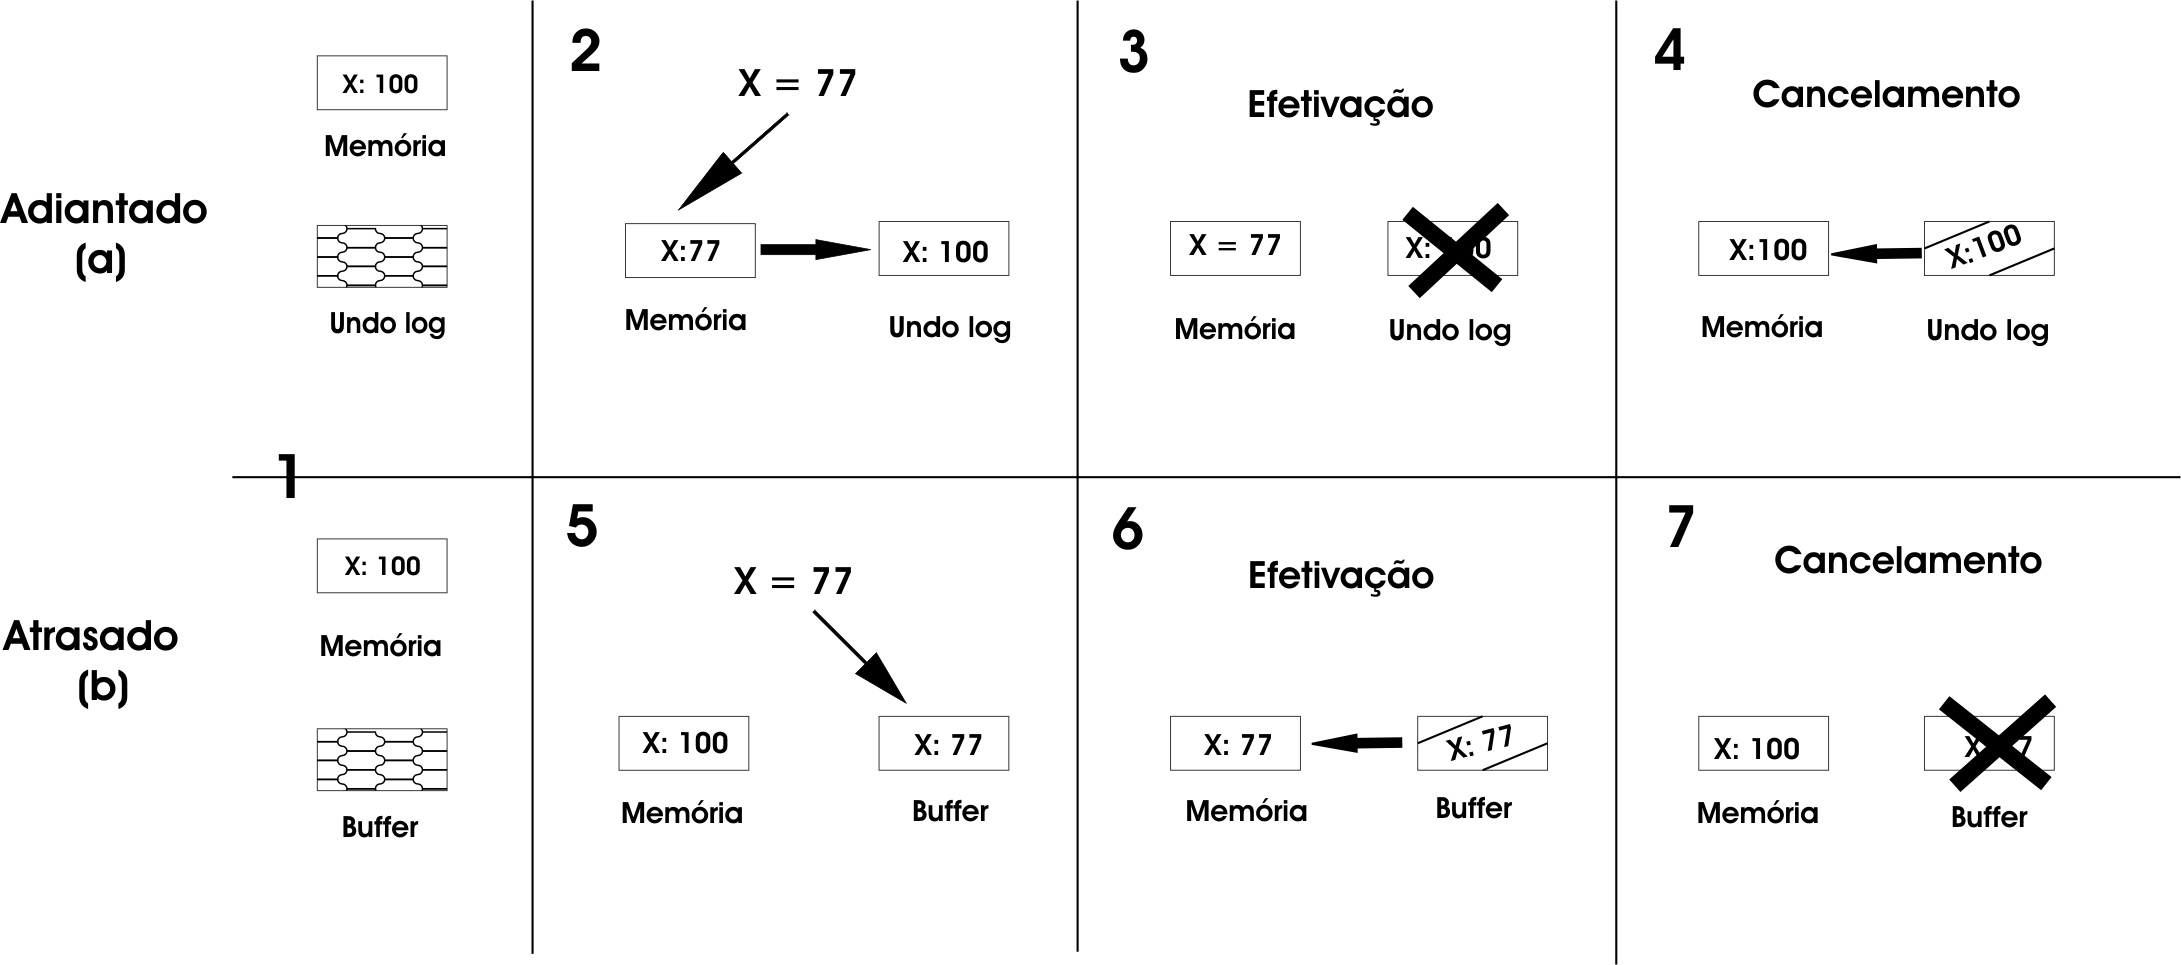
\includegraphics[height=7cm]{images/versionamento.png}
\caption{Exemplo de versionamento adiantado (a) e atrasado (b). Fonte:~\cite{BaldassinTese2009}}
\label{figuraversionamento}
\end{figure}

Existem dois tipos de versionamento de dados:

\begin{itemize}
\item \textbf{Versionamento Adiantado}: como pode ser visto na Figura~\ref{figuraversionamento}~(a), o valor modificado durante a transação é armazenado direto na memória e o valor inicial é armazenado em um \emph{undo log}, para que no caso de \emph{abort} da transação o valor inicial seja restaurado na memória.

\item \textbf{Versionamento Atrasado}: como pode ser visto na Figura~\ref{figuraversionamento}~(b) neste versionamento o valor modificado durante a transação é armazenado em um \emph{buffer} e o valor inicial é mantido na memória até que aconteça um \emph{commit} na transação, onde o valor armazenado no \emph{buffer} é escrito na memória. Caso aconteça o \emph{abort} na transação, o valor do \emph{buffer} é descartado.
\end{itemize}

\section{Detecção de Conflito}

Mecanismos de detecção de conflitos verificam a existência de operações conflitantes durante uma transação. Um conflito ocorre quando duas transações estão acessando um mesmo dado na memória e pelo menos uma das transações está fazendo uma operação de escrita~\cite{BaldassinTese2009}.

Da mesma forma que o versionamento de dados, a detecção de conflito também pode ser de dois tipos:

\begin{itemize}
\item \textbf{Detecção de Conflitos Adiantado}: ocorrem no momento em que duas transações acessam um mesmo dado e uma delas faz uma operação de escrita. Essa operação de escrita é detectada e então uma transação é abortada. Neste tipo de detecção pode ocorrer um problema chamado de \emph{livelock}, quando duas transações geram aborts, desta forma, a execução do programa não progride. A Figura~\ref{figuradeteccaoadiantado} mostra como é feita a detecção de conflitos adiantado.

O Caso~1, mostra a execução sem conflitos, onde as duas transações são executadas sem problemas. Já o Caso~2, mostra o que acontece quando ocorre um conflito, onde T1 lê A e logo depois T2 escreve em A, então o conflito é detectado e T1 é abortada, após ser efetivada T2, a transação T1 consegue ler A sem problema de conflito. Por fim, o Caso~3 mostra a situação de \emph{livelock}, onde as duas transações tentam ler e escrever em A, assim as duas acabam sempre se abortando.

\begin{figure}[!htp]
\centering
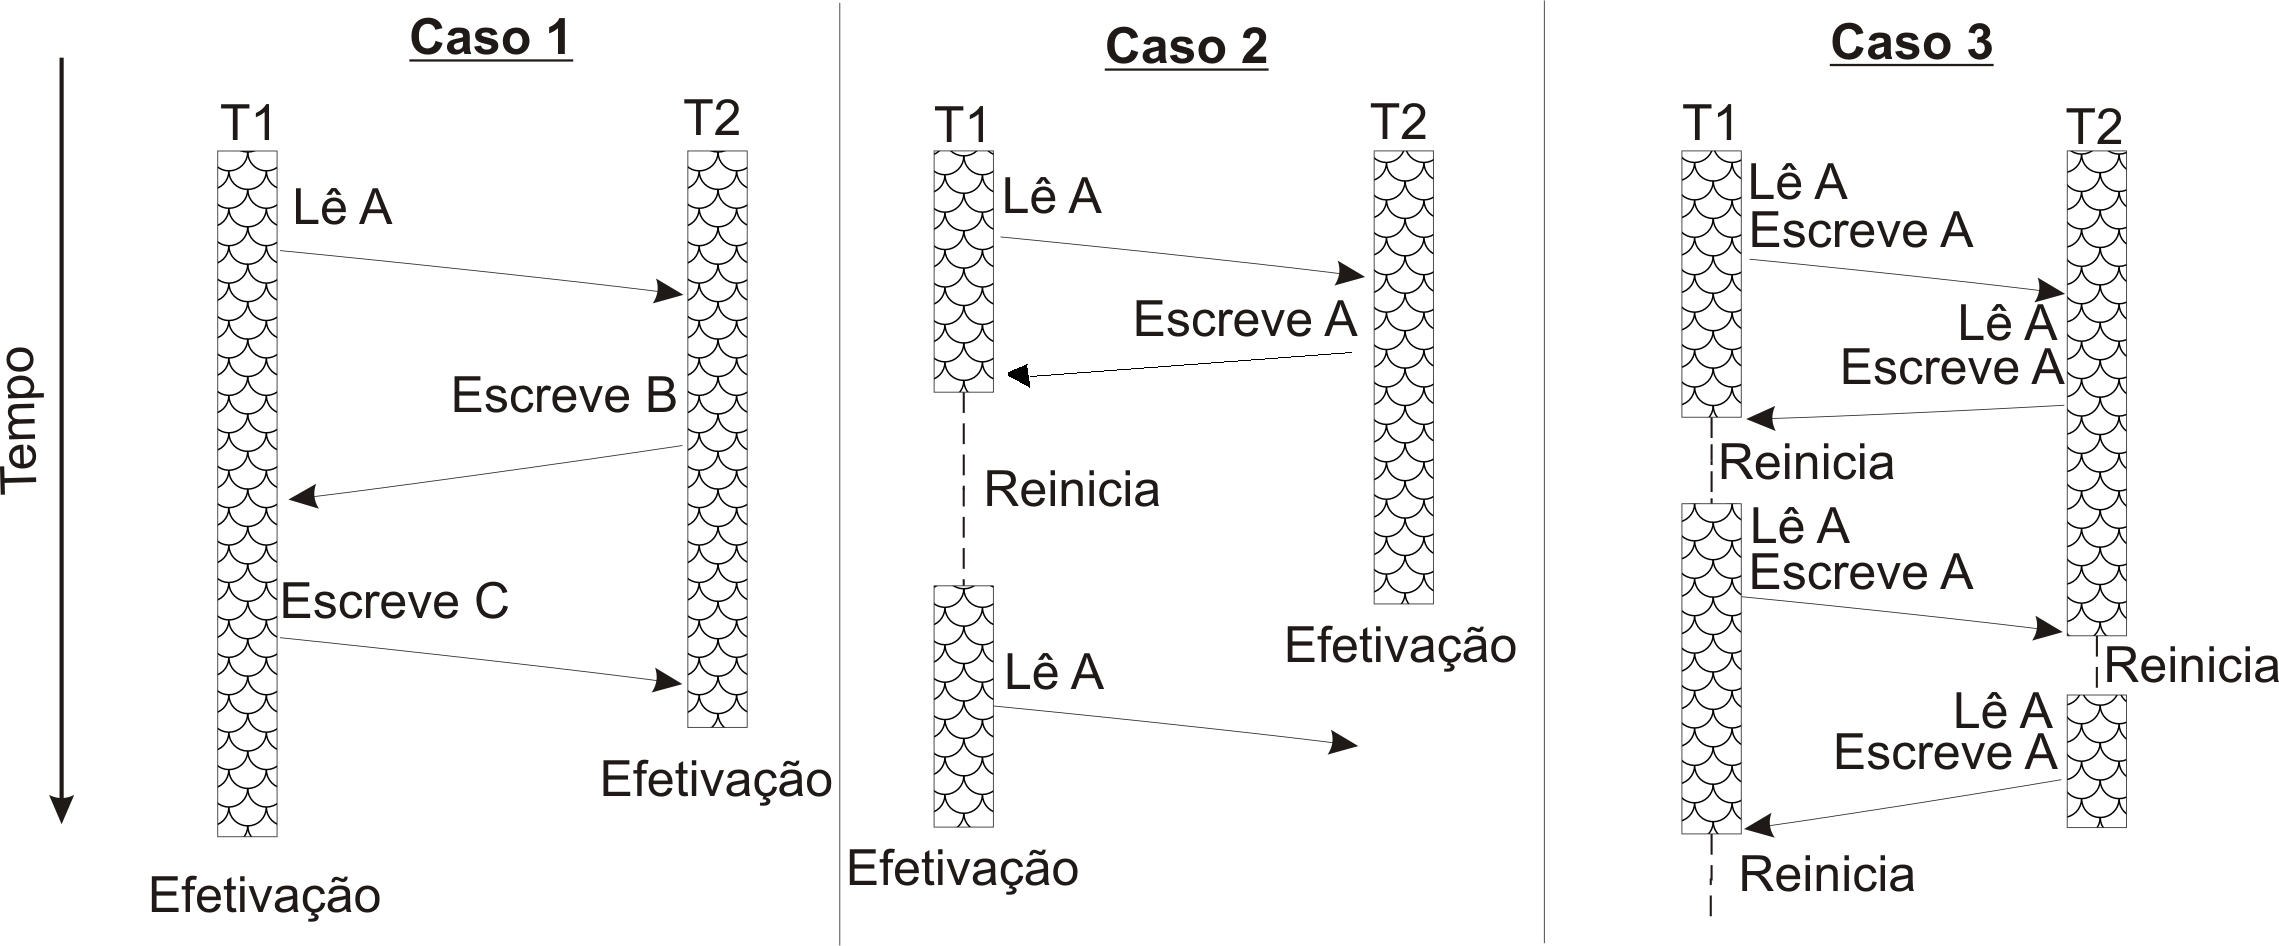
\includegraphics[height=6.5cm]{images/conflitoadiantado.png}
\caption{Detecção de conflitos em modo adiantado. Fonte:~\cite{rigotm}}
\label{figuradeteccaoadiantado}
\end{figure}


\item \textbf{Detecção de Conflitos Atrasado}: Este tipo de detecção de conflito ocorre no final da transação.  Antes da transação ser efetuada, é verificado se ocorreu um conflito. Caso tenha ocorrido, a transação é abortada, se não é efetivada. Para transações muito grandes não é recomendado este tipo de detecção, pois uma transação grande pode ser abortada várias vezes por transações pequenas, assim gastando tempo de processamento desnecessário, este problema se chama \emph{starvation}. A Figura~\ref{figuradeteccaoatrasado} mostra como é feita a detecção de conflitos atrasados.

O Caso~1, mostra as transações acessando dados diferentes, não ocasionando conflitos. No Caso~2, T2 lê A que é escrita por T1. A T2 só nota o conflito quando T1 é efetivado. Logo depois de notar o conflito, T2 é abortada. No Caso~3 não ocorre nenhum conflito, pois T1 lê A antes de T2 escrever. O Caso~4 mostra a situação em que, após ser abortada, T1 volta a executar.
\end{itemize}

\begin{figure}[!htp]
\centering
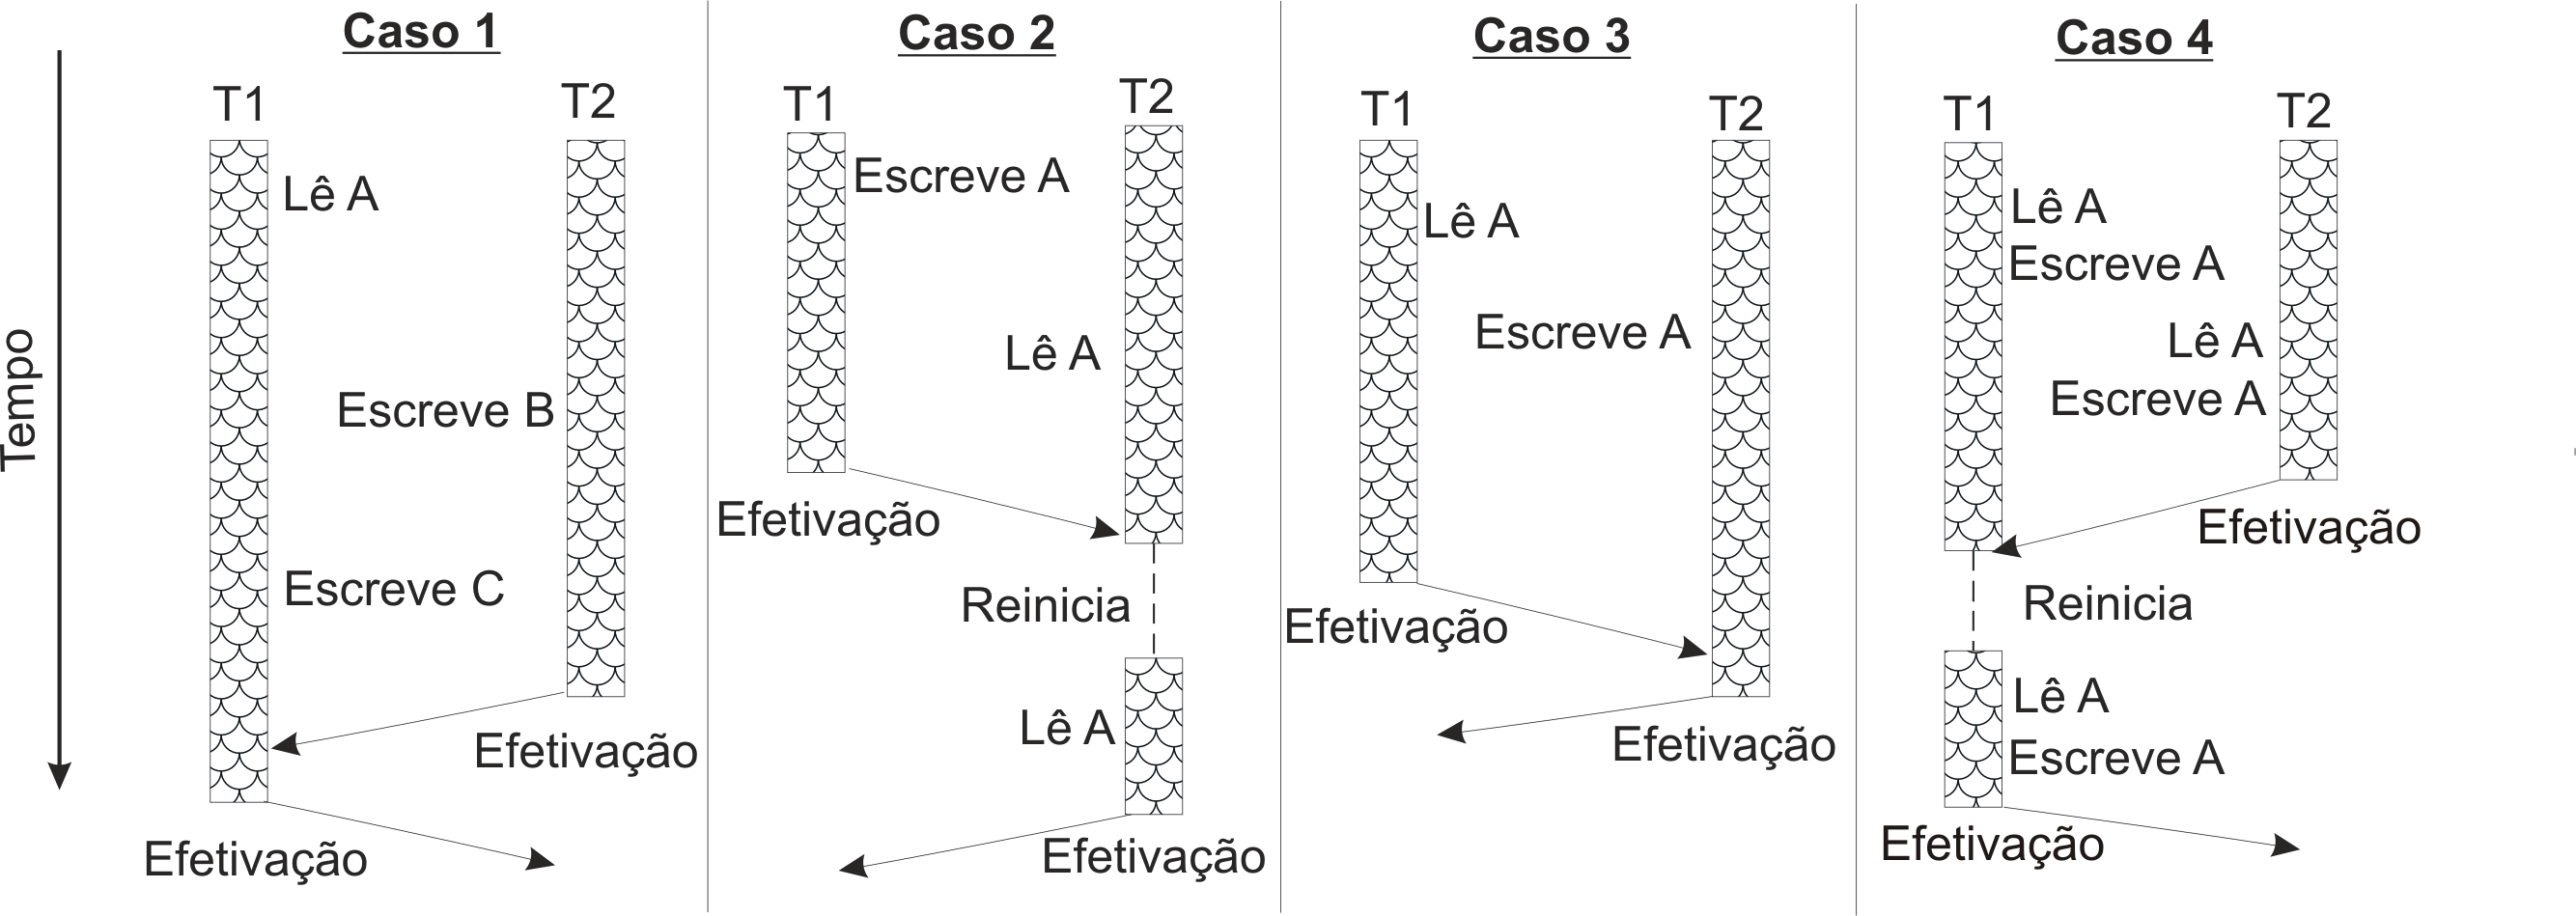
\includegraphics[height=6.5cm]{images/conflitoatrasado.png}
\caption{Detecção de conflitos em modo atrasado. Fonte:~\cite{rigotm}}
\label{figuradeteccaoatrasado}
\end{figure}

Para solucionar o problema de qual transação continuará executando quando ocorre um conflito, é utilizado um gerenciador de contenção~\cite{TM2010}. O gerenciador de contenção é o responsável por decidir quando e qual transação vai ser abortada, isso para garantir que a execução do programa prossiga sem problemas.

\section{TinySTM}

A \emph{TinySTM}~\cite{TINY} é uma implementação de STM para as linguagens C e C++. Ela é uma biblioteca utilizada para escrever aplicativos que usam memórias transacionais para sincronização, em substituição aos tradicionais \emph{locks}.

\subsection{Sincronização e Versionamento}

Na \emph{TinySTM} a sincronização interna das transações é feita a partir de um \emph{array} de \emph{locks} compartilhado que gerencia o acesso concorrente à memória. Cada \emph{lock} é do tamanho de um endereço da arquitetura~\cite{TINY}, e bloqueia vários endereços de memória. O mapeamento é feito por meio de uma função \emph{hash}. A Figura~\ref{figurasincronisacaotinystm} apresenta as estruturas de dados utilizadas nesta implementação.

\begin{figure}[!htp]
\centering
\includegraphics[height=8cm]{images/tinystm.png}
\caption{Estruturas de dados utilizadas na \emph{TinySTM}. Fonte:~\cite{TINY}}
\label{figurasincronisacaotinystm}
\end{figure}

O bit menos significativo é utilizado para indicar se o \emph{lock} está em uso. Se o bit menos significativo indicar que o \emph{lock} não está em uso, nos bits restantes são armazenados um número de versão que corresponde ao \emph{timestamp} da transação que escreveu por último em um dos locais de memória abrangidos pelo \emph{lock}.

Se o bit menos significativo indica que o \emph{lock} está em uso, então nos bits restantes é armazenado um endereço que identifica a transação que está utilizando o dado~(isso utilizando o versionamento adiantado), ou uma entrada no \emph{write set} da transação que está utilizando o dado~(isso utilizando o versionamento atrasado). Em ambos os casos os endereços apontam para uma estrutura que é \emph{word-aligned} e seu bit menos significativo é sempre zero, por isso, o bit menos significativo pode ser utilizado como bit de bloqueio.

Quando utilizado o versionamento atrasado, o endereço armazenado no \emph{lock} permite uma operação rápida para localizar as posições de memória atualizadas abrangidas pelo \emph{lock}, no caso de serem acessados novamente pela mesma transação. Em contraste, a TL2~\cite{tl2} deve verificar o acesso à memória se a transação atual ainda não escreveu neste endereço, o que pode ser caro quando \emph{write sets} são grandes. A leitura depois da escrita não é um problema quando é utilizado o versionamento adiantado porque a memória sempre contém o último valor escrito na memória pela transação ativa.

A \emph{tinySTM} apresenta três estratégias de versionamento distintas que podem ser utilizadas, sendo que duas utilizam versionamento atrasado~(write-back) e uma utiliza versionamento adiantado~(write-through), estas são:

\begin{itemize}
\item \textbf{Write\_Back\_ETL}: esta estratégia implementa o versionamento atrasado com \emph{encounter-time locking}, isso é, o \emph{lock} é adquirido após ocorrer uma operação de escrita e atualiza o \emph{buffer}. O valor é escrito na memória no momento do \emph{commit} da transação;

\item \textbf{Write\_Back\_CTL}: esta estratégia implementa o versionamento atrasado com \emph{commit-time locking}, isto é, ele adquire o \emph{lock} antes de ocorrer um \emph{commit} e atualizar o \emph{buffer}. Assim como no \emph{Write-Back-ETL} o valor é escrito na memória no momento do \emph{commit} da transação;

\item \textbf{Write\_Through}: esta estratégia implementa o versionamento adiantado com \emph{encounter-time locking}, isto é, o valor é escrito direto na memória e mantém um \emph{undo log}, caso ocorra um \emph{abort} na transação é possível restaurar o valor anterior na memória.
\end{itemize}

A \emph{TinySTM} utiliza \emph{Write\_Back\_ETL} como sua estratégia de versionamento padrão.

\subsection{Escritas}

Quando ocorre uma escrita em um local da memória, a transação primeiro identifica o \emph{lock} correspondente ao endereço de memória e lê o valor. Se o \emph{lock} está em uso a transação verifica se é a proprietária do \emph{lock} utilizando o endereço armazenado nos restantes bits de entrada. Caso a transação seja a proprietária então ela simplesmente escreve o novo valor e retorna. Caso contrário, a transação pode esperar por algum tempo ou abortar imediatamente. A \emph{TinySTM} utiliza a última opção como padrão em sua implementação.

Se o \emph{lock} não está em uso, a transação tenta adquiri-lo para escrever o novo valor utilizando uma operação atômica \emph{compare-and-swap}. A falha indica que outra transação adquiriu o \emph{lock} nesse meio tempo, então a transação é reiniciada.


\subsection{Leituras}

Quando ocorre uma leitura na memória, a transação deve verificar se o \emph{lock} está em uso ou se  o valor já foi atualizado concorrentemente por outra transação. Para esse fim, a transação lê o \emph{lock} correspondente ao endereço de memória. Se o \emph{lock} não tem proprietário e o valor~(número de versão) não foi modificado entre duas leituras, então o valor é consistente.

\subsection{Gerenciamento de Memória}

A \emph{TinySTM} utiliza um gerenciador de memória que possibilita qualquer código transacional utilizar memória dinâmica. As transações mantém o endereço da memória alocada ou liberada. A alocação de memória é automaticamente desfeita quando a transação é abortada, já a liberação não pode ser desfeita antes do \emph{commit}. Contudo uma transação pode somente liberar memória depois de adquirir todos os \emph{locks}, assim, um \emph{free} é semanticamente equivalente a uma atualização.

\subsection{Gerenciador de Contenção}

A \emph{TinySTM} implementa quatro estratégias de gerenciador de contenção, estas são:

\begin{itemize}
  \item \textbf{CM\_Suicide}: nesta estratégia a transação que detecta o conflito é abortada imediatamente;

  \item \textbf{CM\_Delay}: esta estratégia assemelhasse a \emph{CM\_Suicide}, porém, espera-se até que a transação que gerou o \emph{abort} tenha liberado o \emph{lock} correspondente ao endereço de memória, então reinicia a transação. Isto porque por intuição a transação que foi abortada irá tentar adquirir o mesmo \emph{lock} novamente, provavelmente falhando em mais de uma tentativa. Esta estratégia aumenta as chances de que a transação tenha sucesso sem gerar um grande número de \emph{aborts}, melhorando o tempo de execução do programa;

  \item \textbf{CM\_Backoff}: também parecida com a \emph{CM\_Suicide}, esta estratégia espera um tempo randômico para reiniciar a transação. Este tempo de espera é escolhido uniformemente ao acaso em um intervalo cujo tamanho aumenta exponencialmente a cada reinicialização;

  \item \textbf{CM\_Modular}: esta estratégia implementa vários gerenciadores de contenção, que são alternados durante a execução. Os gerenciadores utilizados são:

   \begin{itemize}
      \item \textbf{Suicide}: a transação que descobriu o conflito é abortada;

      \item \textbf{Aggressive}: é o inverso da \emph{Suicide}, a transação abortada é a outra e não a que descobriu o conflito;

      \item \textbf{Delay}: a mesma que a \emph{Suicide}, mas aguarda pela resolução do conflito para reiniciar a transação;

      \item \textbf{Timestamp}: a transação mais nova é abortada.
   \end{itemize}
\end{itemize}

A \emph{TinySTM} utiliza a \emph{CM\_Suicide} como sua estratégia padrão de gerenciamento de contenção.

\section{STAMP}
\label{section:stamp}

\emph{Stanford Transactional Applications for Multi-Processing}~\cite{STAMP} é um conjunto de \emph{benchmarks} criado para pesquisa de memórias transacionais, composto por oito \emph{benchmarks}. Apesar de desenvolvido para a STM~TL2, com algumas modificações disponíveis, pode ser usado no \emph{TinySTM}.

%A versão do STAMP utilizada será a 0.9.10.
% O conjunto de \emph{benchmarks} STAMP foi escolhido devido a ele implementar vários \emph{benchmarks}, assim, atingindo uma maior área de aplicações das STM além de ser o conjunto de \emph{benchmark} mais utilizado na pesquisa de STM.

O conjunto de \emph{benchmarks} STAMP implementa vários \emph{benchmarks}, assim, atingindo uma maior área de aplicações das STM e é o conjunto de \emph{benchmark} mais utilizado na pesquisa de STM. Os oito benchmarks disponíveis são:

\begin{itemize}
  \item \textbf{Bayes}: Apresenta uma rede bayesiana de aprendizado;
  \item \textbf{Genome}: Implementa uma aplicação que reconstrói a sequência de um gene a partir de sequências maiores;
  \item \textbf{Intruder}: Simula o Design 5 do \emph{Network Intrusion Detection System}~(NIDS)~\cite{Haagdorens05};
  \item \textbf{Kmeans}:  \emph{K-means} é um algoritmo comumente usado para partição de itens de dados em subconjuntos relacionados;
  \item \textbf{Labyrinth}: Implementa um algoritmo que descobre o menor caminho entre um ponto inicial e um ponto final;
  \item \textbf{SSCA2}: É composto por quatro \emph{kernels}~\cite{Bader05} gráficos dirigidos e ponderados. Estes gráficos são usados em aplicações de biologia computacional;
  \item \textbf{Vacation}: Implementa um sistema de reserva de viagens alimentado por um banco de dados não-distribuído; e
  \item \textbf{Yada}: Implementa o algoritmo de Ruppert~\cite{Ruppert95} para refinamento de malha.
\end{itemize}

Neste trabalho é utilizada a versão 0.9.10 do STAMP para avaliar e comparar a execução da biblioteca de STM TinySTM atual e a utilização do escalonador proposto.

\chapter{Escalonadores}
\label{chapter::escalonadores}

Os algoritmos de escalonamento são responsáveis por garantir a ordem da execução de processos em um sistema operacional. Para programas sequenciais, o escalonador é simples e apenas executa o próximo trabalho da fila. Para programas paralelos o escalonador torna-se complexo, uma vez que, frequentemente há múltiplos trabalhos aguardando execução.

As arquiteturas paralelas atuais fornecem diferentes barramentos para acesso à memória. Algumas pesquisas utilizam escalonadores para fazer com que programas explorem melhor estas arquiteturas. Estudos como \cite{Rodolfo:2014} e \cite{pasqualin2020online} otimizam a execução de programas por meio da redução da latência de acesso à memória e otimização da coerência de cache.

Um problema atual em programas que utilizam STM está na perda de desempenho originada pelos aborts e conflitos de transações. Para solucionar este problema, estudos utilizam escalonadores de STM. Estes escalonadores controlam a execução e a quantidade de threads ativas para reduzir o número de aborts e o tempo de execução das aplicações.

O trabalho apresentado em~\cite{disanzo2017} fornece uma categorização dos escalonadores de STM, na qual os algoritmos são classificados de acordo com suas técnicas.

Está categorização é dividida em algoritmos Baseados em Heurística e algoritmos Baseados em Modelo. Cada categorização possui classificações de acordo com o comportamento de sua técnica.

\begin{itemize}
 \item Baseado em Heurística:
 \begin{itemize}
     \item Feedback: Utiliza o feedback da execução para realimentar sua heurística;
     \item Predição: Utiliza uma predição das informações para tomada de decisão;
     \item Reativo: Só executa sua heurística após determinado comportamento da aplicação ocorrer; e
     \item Heurística Mista: Mescla as classificações anteriores para otimizar a heurística.
 \end{itemize}
 \item Baseado em Modelo:
 \begin{itemize}
     \item Aprendizado de Máquina: Utiliza algoritmos de aprendizado de máquina para tomar decisão;
     \item Modelo Analítico: Monta modelos analíticos para tomar decisão; e
     \item Modelo Misto: Mistura as classificações acima para otimizar a heurística.
 \end{itemize}
\end{itemize}

% \section{Categorias}

A tabela~\ref{tab:compare} apresenta as classificações dos principais algoritmos revisados na bibliografia durante o desenvolvimento deste trabalho.

\begin{table}[]
\footnotesize
\centering
\caption{Algoritmos e técnicas de escalonamento}
\label{tab:compare}
\begin{tabular}{l|l}
\hline
Escalonador & Técnica \\ \hline
ATS & Feedback \\
% Probe & Feedback \\
% F2C2 & Feedback \\
Shrink & Predição \\
% SCA & Predição \\
CAR-STM & Reativo \\
% RelSTM & Reativo \\
LUTS & Heurística Mista \\
ProVIT & Heurística Mista \\
% SAC-STM & Aprendizado de Máquina \\
% CSR-STM & Modelo Analítico \\
% MCATS & Modelo Analítico \\
% AML & Modelo Misto \\
STMap & Predição \\
\hline
\end{tabular}
\end{table}

\section{ATS}

\emph{Adaptive Transaction Scheduling}~(ATS)~\cite{ats2008} foi um dos primeiros trabalhos a apresentar um escalonador de MT para trabalhar junto com gerenciador de contenção.

O ATS utiliza um valor para tomada de decisão denominado CI (Contention Intensity), cada thread em execução possui seu próprio CI. O CI é calculado cada vez que ocorre um commit ou um abort e é zerado a cada início de transação.

O escalonador utiliza o valor do CI em sua tomada de decisão. Quando o valor do CI ultrapassa um limiar pré definido, a thread é colocada em uma única fila para garantir uma execução de forma serial.

\section{CAR-STM}

\emph{Collision Avoidance and Resolution}~(CAR-STM)~\cite{carstm2008} foi desenvolvido para evitar que conflitos já existentes voltem a ocorrer. Para isto é apresentado duas heurísticas de gerenciamento.

A primeira heurística é denominada Básica e busca executar de forma serial as transações conflitantes sem manter um histórico da execução. A segunda, denominada Permanente, busca manter um histórico das transações que conflitaram e executá-las de forma serial.

\begin{itemize}
 \item Básica: Quando detectado um conflito, a transação mais recente é abortada e migrada para fila da transação conflitante, assim sua execução será serializada com a transação conflitante.
 \item Permanente: Quando uma transação Tb aborta em relação a Ta, Tb é migrado para fila de Ta e sua ordem de execução será Ta -> Tb. Caso a transação Ta conflite e aborte em relação a Tc, Ta deverá ser migrada para fila de Tc carregando sua dependência Ta -> Tb.
\end{itemize}

\section{LUTS}

\emph{Light-Weight User-Level Transaction Scheduler}~(LUTS)~\cite{Nicacio2012} apresenta um escalonador que busca evitar a ociosidade de um núcleo após a serialização de uma transação.

Para isto, cada thread é representado internamente por um Registro de Contexto em Execução (RCE). No início da execução o escalonador cria uma fila de RCEs para serem executados no futuro.

Assim, o LUTS dispara um RCE por núcleo, e utiliza a fila para não disparar mais RCEs que núcleos disponíveis. Cada RCE disparado é convertido em uma thread de sistema que executa um conjunto de transações.

Na tentativa de evitar conflitos, o LUTS apresenta uma forma dinâmica para solucioná-los, considerando transações curtas e transações longas. Para definir o tamanho da transação é utilizada a contagem de ciclos da mesma, onde a partir de 100 mil ciclos é caracterizada uma transação longa.

Para transações curtas, a heurística utilizada é similar a do ATS, o escalonador calcula a intensidade de conflito da transação e serializa esta quando o cálculo ultrapassa um limiar. Porém o LUTS escolhe outra transação para substituir a atual.

Para transações longas, a heurística é mais elaborada, utilizando três metadados globais:

\begin{itemize}
 \item  activeTx: Um vetor de tamanho igual ao total de núcleos disponíveis, usado para armazenar o identificador da transação que está sendo executada.
 \item conflictTable: Uma tabela do histórico de conflitos, cada linha armazena um conjunto de transações dada pelo activeTx, e cada coluna armazena a probabilidade de conflito.
 \item bestTx: Um vetor que sumariza a melhor transação a ser executada para cada núcleo.
\end{itemize}

Quando uma transação realiza um commit ou abort o escalonador se encarrega de atualizar a conflictTable na sua respectiva linha, aumentando ou diminuindo sua probabilidade de conflito.

Para evitar percorrer a conflictTable no início de cada transação o LUTS percorre a bestTx e seleciona qual transação deve executar. Quando a conflictTable é atualizada o escalonador atualiza a bestTx.

\section{Shrink}

\emph{Shrink}~\cite{shrink2009} apresenta um escalonador que busca minimizar a ocorrência de aborts com base nos conjuntos de leituras e escritas de cada thread.

O escalonador é baseado em predição e usa como heurística os acessos à memória das transações executadas anteriormente. Para evitar \emph{overhead} em sua execução o Shrink avalia os acessos apenas se existir uma alta contenção no sistema.

No início de cada transação o escalonador avalia se a relação entre commit e abort é superior a um limiar predefinido. Se esse valor for superior ao limiar o escalonador considera que o sistema possui uma alta contenção e ativa a heurística para serializar as transações em execução.

Cada thread possui um conjunto dos acessos de leitura e escrita realizados pelas transações Quando uma transação iniciar com um sistema de alta contenção esse conjunto de leitura e escrita é verificado, se outra thread em execução possuir um conjunto semelhante o escalonador assume que há uma alta chance da transação abortar.

Para que a transação não aborte, a thread que iniciaria a transação é bloqueada até o fim da transação na thread em execução, assim o Shrink busca forçar a serialização das execuções.

\section{ProVit}

O escalonador \emph{ProVIT}~\cite{rito2015} fornece uma abordagem otimista da execução, evitando considerar que toda transação que abortou irá abortar novamente na sequência.

Assim como o LUTS, o ProVIT avalia o tamanho das operações atômicas para aplicar sua heurística. Porém no ProVIT mais de uma heurística pode estar ativa ao mesmo tempo.

Também foi apresentada a observação de que duas transações conflitantes, de leitura e escrita, podem efetuar o commit dependendo da ordem, se o commit for efetuado primeiro pela transação de leitura, a de escrita não será conflitante.

Operações atômicas longas utilizam uma política baseada em grão fino para melhorar a precisão da predição e evitar a reexecução de transações. Essa predição utiliza como base o conjunto de leitura das transações já executadas.

Se uma transação efetua um abort o escalonador marca esta transação como Very Important Transaction (VIT) e copia seu conjunto de leitura para uma lista auxiliar global.  Quando uma transação tenta efetuar um commit, ela verifica a lista global para garantir que não há conflito entre os conjuntos de escrita e leituras da lista global.

Caso haja conflito entre a transação e alguma VIT, o commit é adiado por um tempo pré-determinado. Assim, o escalonador tenta garantir que as VITs não abortem novamente. Caso não haja conflito o commit é realizado.

Nas operações atômicas curtas a heurística evita a validação com base na intersecção para não adicionar \emph{overhead} desnecessário. Sendo assim, ela apresenta uma ideia similar a do ATS, onde é utilizada uma métrica de decisão para serializar as transações.

Para definir quando uma transação será serializada, o escalonador utiliza um valor calculado em tempo de execução denominado Tempo Perdido (TP). Cada operação atômica possui seu próprio TP, que é calculado com base em um valor pré-definido e a quantidade de reexecução da transação e seu TP anterior.

Toda operação atômica começa com TP igual a zero e é executada livremente, conforme o TP aumenta o ProVit se encarrega de serializar as transações reduzindo a concorrência até o ponto em que somente uma transação poderá ser executada por vez.

Para definir se uma operação atômica é curta ou longa foi implementada uma política de definição, onde toda operação atômica inicia sua execução como curta. Quando uma transação finaliza o escalonador atualiza seu conhecimento sobre as operações atômicas com base no TP.

Uma operação atômica é considerada longa quando o tamanho médio do seu conjunto de leitura for maior que um limite pré-definido. Assim, o tamanho da operação atômica é baseado nas operações de leitura e não no tempo de execução.

\section{STMap}

O \emph{STMap}~\cite{pasqualin2020online} utiliza o mecanismo de sharing-aware thread mapping para aplicações STMs. Esse mecanismo usa informações sobre quais threads estão acessando os mesmos dados compartilhados e tenta mapear de forma que as threads fiquem próximas na arquitetura onde está sendo executada.

Em tempo de execução o STMap coleta dados sobre os acessos compartilhados entre as threads, esses dados são usados para calcular um mapeamento que tenta deixar estas threads próximas na arquitetura para compartilhar cache, visto que acessam um mesmo dado compartilhado.

A coleta de dados é realizada em tempo de execução quando ocorre uma escrita ou leitura dentro de uma transação, esse endereço de leitura ou escrita é comparado com os endereços utilizados pelas outras transações. Se esse endereço é usado por outra transação o STMap incrementa uma matriz de comunicação com essas informações.

A matriz de comunicação possui como tamanho o mesmo número de threads em execução. Supondo que a transação tx executada pela thread T1 manipule o mesmo endereço que a transação ty da thread T2, a transação tx descobre o ID da thread T1 e da thread T2 e incrementa o valor da matriz de comunicação nas posições respectivas aos IDs.

Essa matriz é utilizada para caracterizar as transações e mapear a arquitetura em relação às threads, assim sendo possível agrupar as threads por nós de processamento para otimizar a execução e aproveitar ao máximo a coerência de cache.

\section{Discussão}

Máquinas \emph{NUMA} têm a vantagem de agregar maior paralelismo ao adicionar mais processadores sem aumentar o gargalo de acesso ao barramento. Sua arquitetura é feita para que os processadores não utilizem o mesmo barramento de acesso à memória como é feito em arquiteturas \emph{UMA}.

As arquiteturas \emph{NUMA} possuem múltiplos núcleos dispostos em conjuntos de processadores (nós), a memória é fisicamente composta por vários bancos de memória, podendo estar cada um deles vinculados a um nó e a um espaço de endereçamento compartilhado. Quando o processador acessa a memória que está vinculada a si, diz-se que houve um acesso local. Se o acesso for à memória de outro processador, diz-se que ocorreu um acesso remoto. Os acessos remotos são mais lentos que os acessos locais, uma vez que é necessário passar pela rede de interconexão para que se consiga chegar ao dado localizado na memória remota~\cite{Rodolfo:2014}.

Os escalonadores de STM atuais buscam reduzir o número de conflitos para reduzir a quantidade de reexecução das transações. Para isto estes escalonadores implementam filas de execução e migração de threads que tornam serial a execução das transações conflitantes, como nos trabalhos apresentados em~\cite{shrink2009},~\cite{Nicacio2012}, e~\cite{rito2015}.

Algoritmos NUMA-Aware avaliam as diferentes características da arquitetura que a aplicação está executando. Possuindo conhecimento das diferentes latências de acesso à memória, esses algoritmos podem extrair o máximo de recurso da máquina. Assim, alguns algoritmos NUMA-Aware avaliam os conjuntos de leitura e escrita das aplicações para decidir qual é o melhor nó de execução para a thread, ou quando deve ser migrada a página de memória. Outros utilizam uma matriz de comunicação para fazer um mapeamento de threads e assim otimizar sua execução, como é feito em~\cite{pasqualin2020thread}.

Os escalonadores de STM atuais não consideram a arquitetura e seu custo de acesso à memória para serializar as execuções. Alguns escalonadores de STM avaliam os conjuntos de leitura e escrita apenas com interesse em reduzir o número de conflitos, como é visto em~\cite{shrink2009}.

O LTMS, diferente de outros trabalhos, é um escalonador que avalia as características da arquitetura, e em tempo de execução monta uma matriz de comunicação com base nas leituras e escritas realizadas pelas threads. Está matriz de comunicação é utilizada para avaliar o custo de acesso à memória e migrar as threads em execução entre as filas, buscando diminuir os números de conflitos por meio da serialização das transações e otimizar a execução aproveitando a melhor distribuição das tarefas na arquitetura NUMA, reduzindo assim a latência de acesso à memória.

A tabela~\ref{tab:compare_ltms} apresenta uma comparação entre as principais características do LTMS e os escalonadores apresentados neste trabalho, a tabela busca entender as diferenças que o escalonador fornece para aplicações paralelas que utilizam STM.

\begin{table}[]
 \footnotesize
 \centering
 \caption{Comparativo entre os escalonadores apresentados}
 \label{tab:compare_ltms}
 \begin{tabular}{l|l|l|l|l|l|l|l}
 \hline
  Escalonadores                     & LTMS    & ATS      & Shrink   & LUTS  & ProVIT  & STMap     & CAR-STM \\ \hline %escalonadores
  Distribuição inicial de threads   & Sim     & Não      & Não      & Sim   & Não     & Não       & Não \\
  Coleta de dados por threads       & Sim     & Não      & Sim      & Não   & Não     & Sim       & Não \\
  Migração entre filas              & Sim     & Não      & Não      & Não   & Não     & Não       & Sim \\
  Avalia a arquitetura              & Sim     & Não      & Não      & Não   & Não     & Sim       & Não \\
  Técnica de escalonamento          & Reativo & Feedback & Predição & Mista & Mista   & Predição  & Reativo  \\
 \hline
 \end{tabular}
\end{table}

\chapter{LTMS - Lups Transactional Memory Scheduler}
\label{chapter::ltms}

Memórias transacionais fornecem um nível maior de abstração para o desenvolvimento de programas paralelos, e conforme descrito no capítulo~\ref{chapter::escalonadores}, existem vários trabalhos que focam em desenvolver escalonadores que compreendem a aplicação para extrair melhor desempenho.

Porém, os escalonadores atuais não consideram as diferenças entre as arquiteturas paralelas existentes. O escalonador LTMS, proposto neste trabalho, se propõe a avaliar a aplicação e a arquitetura em tempo de execução para tirar proveito do paralelismo existente.

O LTMS foi desenhado para acompanhar toda execução de uma aplicação que utiliza STM. Sendo assim, inicialmente ele provê filas de execução e implementa estratégias de distribuição de threads entre as filas no início da aplicação. Além disso, para entender a aplicação são coletados os endereços de escrita e leitura, e os números de aborts e commits das threads e transações em tempo de execução, estes dados são utilizados nas heurísticas que definem quando uma thread deve ser migrada para reduzir latência de acesso a memória ou reduzir a contenção gerada na aplicação.

\section{Escalonador}

O LTMS é um escalonador de STM NUMA-Aware que identifica as características da arquitetura e do programa em tempo de execução para extrair um desempenho melhor da máquina utilizada. O escalonador opera em três estágios apresentados na Figura~\ref{ltms_estagios}, sendo eles, a inicialização do sistema, a coleta de dados em tempo de execução e a migração de threads.

\begin{figure}[htbp]
\centering 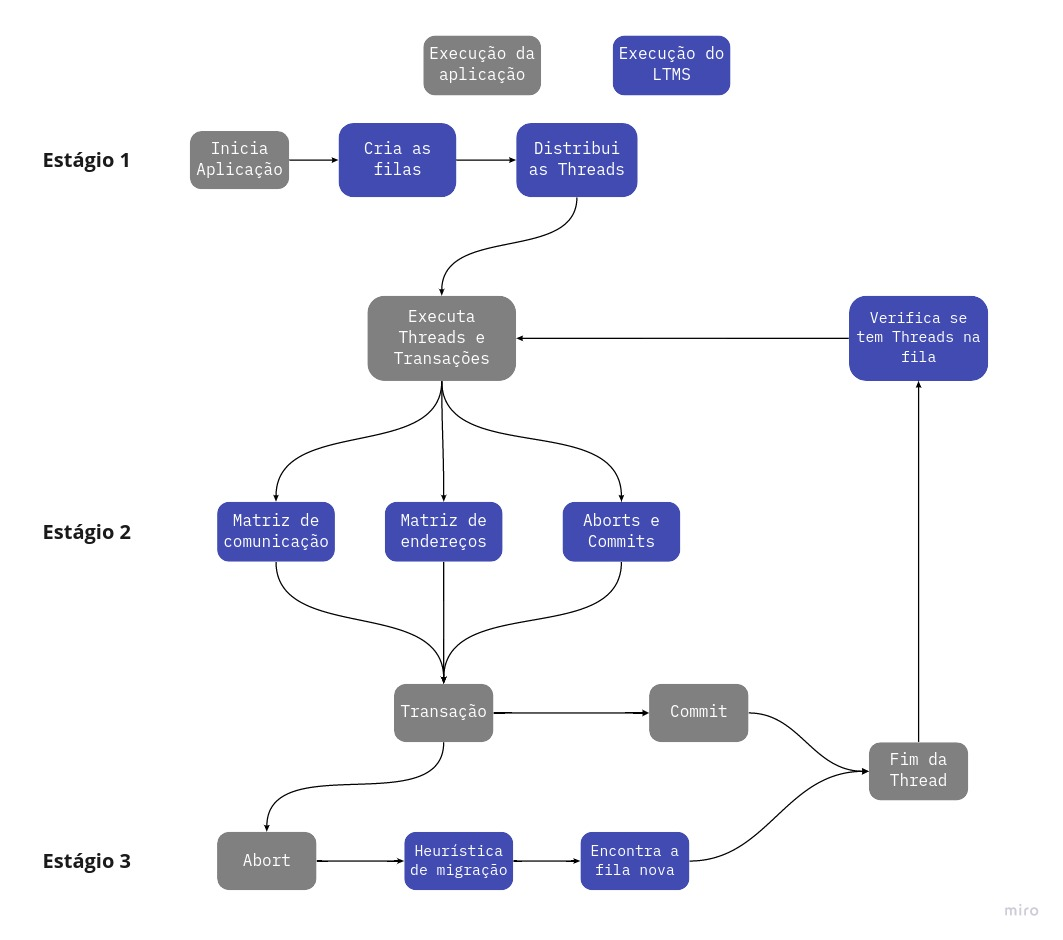
\includegraphics[scale=.3]{images/LTMS1}
\caption{Fluxo de estágios do LTMS}
\label{ltms_estagios}
\end{figure}

\begin{itemize}
 \item Inicialização do sistema: Inicialmente associa filas de execução aos processadores e implementa uma estratégia configurável de distribuição inicial de threads;
 \item Coleta de dados em tempo de execução: Em tempo de execução, são coletadas informações de acesso a memória e a quantidade de commits e aborts feitas pelas transações; e
 \item Migração de Threads: Quando transações abortam, utiliza heurísticas baseadas nos dados coletados, para decidir se as threads devem ser migradas para outras filas.
\end{itemize}

\subsection{Inicialização do sistema}
\label{inicializacao}

Como é possível visualizar na Figura~\ref{ltms_generic} o escalonador LTMS é inicializado junto com a aplicação. O escalonador é responsável por ler as característica da arquitetura e criar filas de execução com base nas threads da aplicação e no número de \emph{cores} disponíveis. O LTMS fornece uma biblioteca de threads integrada a STM que provê todos os recursos necessários para o desenvolvimento das aplicações. Quando uma thread é criada ela fica disponível para o escalonador distribuir ela entre as filas com base em uma estratégia de distribuição.

\begin{figure}[htbp]
\centering 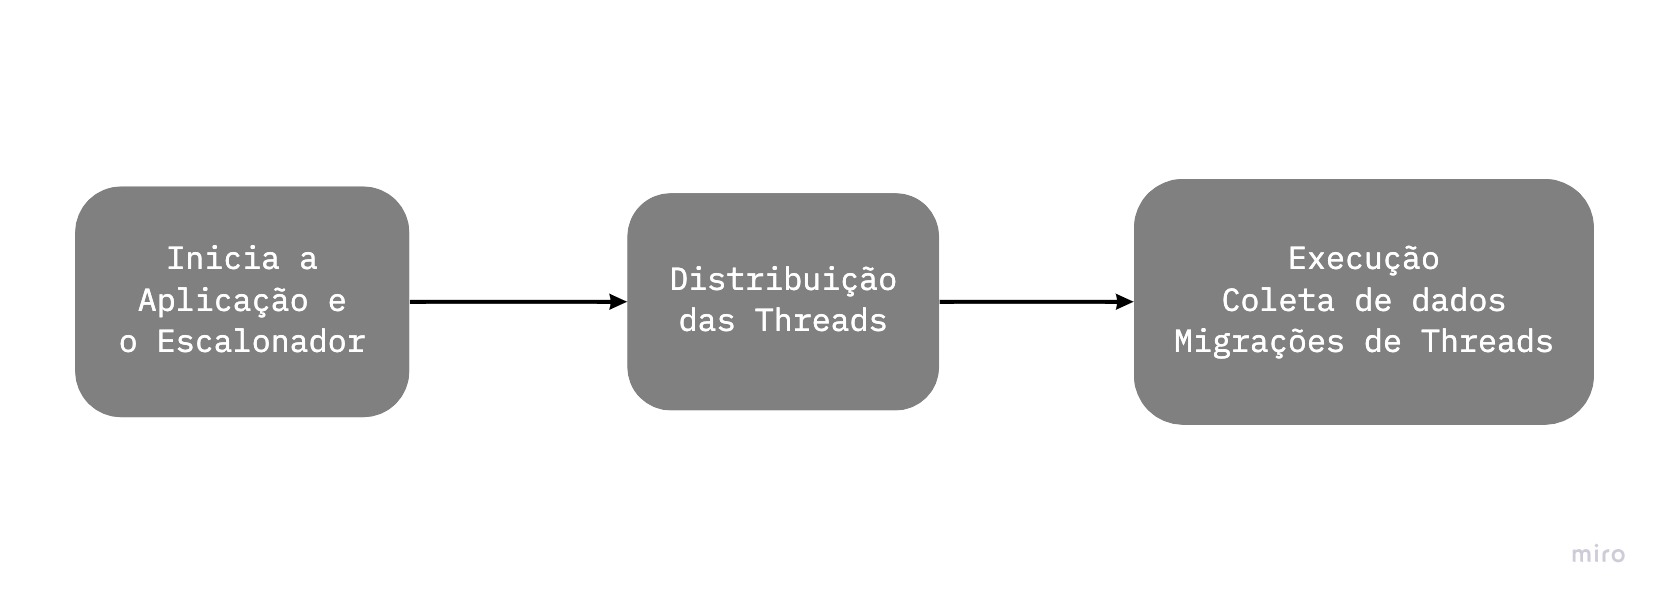
\includegraphics[scale=.25]{images/ltms_generic}
\caption{Fluxo de execução do LTMS}
\label{ltms_generic}
\end{figure}

Ao inicializar uma aplicação o número de threads utilizados é passado para o escalonador na chamada de sua biblioteca de threads, assim, o LTMS compara o número de threads da aplicação com a quantidade de \emph{cores} da máquina, se o número de threads da aplicação for maior que o número de \emph{cores} o LTMS cria uma fila para cada core, como visto na Figura~\ref{queue_core}.

\begin{figure}[htbp]
\centering
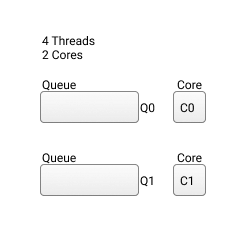
\includegraphics[scale=.65]{images/Queue_core.png}
\caption{Criação das filas de execução com base nos \emph{cores}}
\label{queue_core}
\end{figure}

Se a quantidade de threads da aplicação for menor que o número de cores disponível na arquitetura, o LTMS cria a mesma quantidade de filas que a quantidade de threads, fixando um core por fila e distribuindo uma thread por fila.
% como visto na figura~\ref{queue_thread}

% \begin{figure}[htbp]
% \centering
% 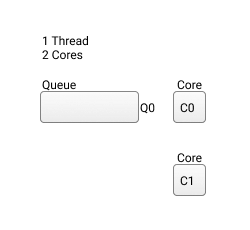
\includegraphics[scale=.8]{images/Queues_thread.png}
% \caption{Criação das filas de execução com base nas threads}
% \label{queue_thread}
% \end{figure}

Após a criação das filas de execução, conforme descrito, as threads criadas na aplicação são distribuídas com base em uma estratégia de distribuição cíclica. O escalonador foi desenhado para que a distribuição seja baseada em chunks, onde o tamanho de um chunk seja o número de threads disposto para cada fila, o LTMS permite ao desenvolvedor definir o tamanho do chunk para testar diferentes distribuições de threads. Para este trabalho foram utilizados dois tamanhos de chunks junto à estratégia de distribuição.

A primeira estratégia implementada, denominada Sequential, possui o tamanho de chunk um, assim distribuindo uma thread por fila até a conclusão de todas threads disponíveis. A Figura~\ref{sequential} traz como exemplo 4 threads e 2 cores, neste caso serão criadas uma fila para cada core.

O escalonador executará a primeira fase de distribuição, colocando uma thread para cada fila existente. Após a primeira fase o escalonador verifica se ainda possui threads a serem distribuídas, caso haja threads o LTMS repete a distribuição em uma segunda fase, até acabarem as threads.

Neste cenário a Fila intitulada Q0 fica com as threads t0 e t2, e a fila Q1 fica com as threads t1 e t3. Importante destacar que o LTMS alocou a thread t0 em Q0 e depois alocou t1 em Q1, então voltou a execução para alocar t2 em Q0 e t3 em Q1.

\begin{figure}[htbp]
\centering
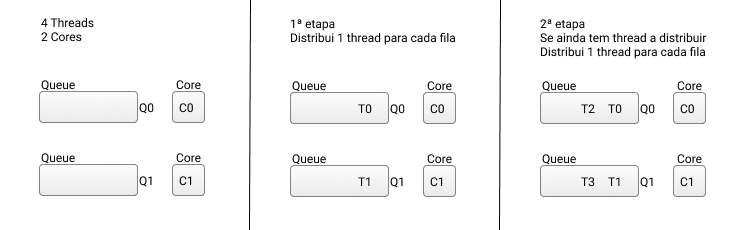
\includegraphics[scale=.6]{images/Queue_one.png}
\caption{Estratégia Sequential de distribuição de threads}
\label{sequential}
\end{figure}

A segunda estratégia, denominada Chunks, o tamanho do chunk é determinado pela razão entre a quantidade de threads e a quantidade de filas. No exemplo apresentado na Figura~\ref{chunks} temos o mesmo cenário de filas, cores e threads apresentados anteriormente.

Na primeira fase de distribuição o escalonador aloca duas threads, o primeiro chunk, na primeira fila, após isto a segunda fase aloca o próximo chunk na segunda fila. Se existir mais chunks o escalonador segue sua distribuição entre as filas disponíveis. Caso haja um número impar de threads para distribuir o escalonador agrupa as threads restantes em um chunk que será alocado na fila em que a distribuição parou.

Neste cenário o LTMS aloca na fila Q0 as threads t0 e t1, e na fila Q1 as threads t2 e t3. Importante notar que o primeiro chunk é composto por t0 e t1 e t2 e t3 representam o segundo chunk.

\begin{figure}[htbp]
\centering
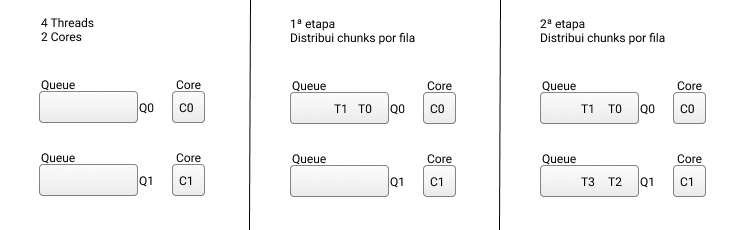
\includegraphics[scale=.6]{images/Queue_chunks.png}
\caption{Estratégia Chunks de distribuição de threads}
\label{chunks}
\end{figure}


\subsection{Coleta de dados em tempo de execução}
\label{coleta}

Durante a execução da aplicação, o escalonador se encarrega de coletar dados de sua execução e da arquitetura utilizada para otimizar a redistribuição de threads entre as filas existentes caso ocorram aborts nas transações. Entre os dados coletados estão os acessos à memória, a quantidade de aborts e a quantidade de commits realizados pelos threads, também são coletadas informações sobre os nós NUMA existentes na arquitetura e os custos de latência existentes.

Os dados coletados sobre os acessos à memória fornecem insumos para duas matrizes, uma matriz de comunicação e uma matriz de endereços. Estas matrizes serão utilizadas nas heurísticas de migração para definir o grau de relação entre as filas de execução para reduzir os conflitos após uma migração de threads entre as filas.

A matriz de comunicação fornece insumos sobre a quantidade eventos de comunicação entre dois threads, onde cada posição da matriz representa a quantidade de comunicação entre pares de threads. Quando dois threads acessam o mesmo endereço, é gerado o evento, e a matriz guarda a quantidade de eventos de comunicação que foram gerados.

Para evitar \emph{overhead} a coleta de dados da matriz de comunicação ocorre por amostragem, neste trabalho utilizamos 1 a cada 100 acessos por thread para acionar o contador, esta abordagem é baseada nos experimentos apresentados nos trabalhos~\cite{pasqualin2020online}. 

% \todo{um flowchart fig25 pg79 do douglas}
A matriz de endereços por sua vez, possui para cada posição uma tabela hash que contem uma estrutura de chave e valor. Esta estrutura utiliza como chave o endereço de memória acessado e como valor, a quantidade de acessos que este endereço recebeu.Quando duas threads acessam o mesmo endereço de memória, um evento é disparado, este evento busca na tabela hash a chave com endereço que foi acessado e incrementa o valor de acessos que este endereço recebeu.

% O evento disparado pelo acesso em comum utiliza este array para verificar e armazenar na matriz o endereço com maior valor.

% Os valores da matriz de endereços são os endereços de memória acessados mais vezes entre dois threads, e assim como na matriz de comunicação os identificadores dos threads são as posições da matriz. 
% Assim, se a thread com id 0 e a thread de id 1 possuem mais acesse em comum com o endereço 0xbff6f36c, o valor da matriz de endereços na posição \emph{matrixAddress[0][1]} será 0xbff6f36c.

% Para montar a matriz de endereços foi utilizado o mesmo sistema de amostragem apresentado anteriormente, no momento do armazenamento o endereço avaliado é armazenado em uma fila que é ordenada pela quantidade de acessos que o endereço recebeu, o endereço com maior número de acessos é armazenado na matriz de comunicação.

O LTMS também fica encarregado de coletar dados sobre o comportamento das transações. Durante sua execução uma thread pode ter n transações que geram aborts e commits. O escalonador mantém em cada thread um contador para os commits e um para os aborts. Esse contador mantém o histórico de commits e aborts de uma thread que será utilizado para identificar o índice de contenção da thread.

\subsection{Migração de Threads}
\label{migracao}

O LTMS fornece um sistema de migração de threads entre as filas existentes, esse sistema entra em ação após a ocorrência de um abort e busca agrupar as threads conflitantes com intuito de serializa-las para evitar conflitos futuros. O sistema de migração é dividido em duas etapas, a identificação da fila para qual o thread será migrado e a heurística de migração que define se a migração irá acontecer.

A Figura~\ref{migration} ilustra a função de migração denominada~\emph{migrateThread}. Esta função é executada após a ocorrência de um abort, a função~\emph{findBestQueue} identifica a fila para qual podemos efetuar a migração e a função~\emph{okToMigrate} utiliza uma heurística que determina se devemos migrar a thread atual. Caso a thread deva ser migrada, a thread é adicionada à fila de execução para qual deseja-se migrá-la. Caso a thread não deva ser migrada, a função retorna para operação de abort e segue a execução utilizando o gerenciador de contenção.

\begin{figure}[htbp]
 \centering
 \begin{lstlisting}
   migrateThread(thread) {
     if (okToMigrate(thread))
       findBestQueue(thread).push();
   }
 \end{lstlisting}
 \caption{Função de migração}
 \label{migration}
\end{figure}

A etapa de heurística de migração, representada na função~\emph{okToMigrate} e apresentada na Figura~\ref{migration}, avalia se a thread que gerou o abort está apta a ser migrada. O LTMS permite que diferentes heurísticas de migração sejam desenvolvidas e acopladas a ele.  Para este trabalho foram desenvolvidas duas heurísticas de migração, que avaliam os dados coletados para tomar a decisão de migrar a thread. Estas heurísticas foram denominadas \emph{threshold} e \emph{latency} e são apresentadas nas Figuras~\ref{threshold} e~\ref{latency}.

A primeira heurística, denominada threshold, avalia o nível de contenção apresentado pela thread em tempo de execução, esse nível de contenção é medido pela razão entre os aborts e commits realizados pela thread, onde um resultado alto indica uma maior contenção ocasionada pelos aborts. Para realizar uma migração utilizando esta heurística o LTMS executa a função apresentada na Figura\ref{threshold}.

A função \emph{thresholdHeuristic} apresentada na Figura~\ref{threshold} calcula o índice de contenção dado pela razão dos aborts e commits realizados pela thread e avalia se o índice de contenção é maior que um valor limiar. Se o índice de contenção for maior que o limiar a função permite a migração da thread, se o valor do índice de contenção ficar abaixo do limiar a thread não deve ser migrada.

O limiar denominado~\emph{threshold} é uma constante definida pelo desenvolvedor que indica o nível máximo de contenção aceito pela aplicação. Um valor baixo para o limiar gera mais migrações, o que proporciona maior serialização do sistema, reduzindo assim os aborts e aumentando tempo de execução, enquanto um limiar muito alto mantém o paralelismo mas aumenta o número de aborts. Para está dissertação foram executados testes para entender o comportamento do LTMS utilizando diferentes valores no threshold. O valor de threshold que apresentou o melhor desempenho com os benchmarks testados foi o valor de 0,8. Este valor indica que quando a thread possuir um índice de contenção de 80\% o LTMS deve efetuar a migração desta thread.

\begin{figure}[htbp]
 \centering
 \begin{lstlisting}
   bool thresholdHeuristic(thread) {
     return thread.aborts/thread.commits >= threshold
   }
 \end{lstlisting}
 \caption{Heurística de migração threshold}
 \label{threshold}
\end{figure}

A segunda heurística de migração, denominada \emph{latency}, avalia a latência de acesso à memória entre os nós da filas envolvidas na migração e o endereço de memória mais acessado pela thread. Para realizar uma migração utilizando esta heurística o LTMS executa a função denominada~\emph{latencyHeuristic} apresentada na Figura\ref{latency}.

A função \emph{latencyHeuristic} busca na matriz de endereços qual o endereço de memória em comum é mais acessado pelas filas. A função também consulta quais os nós NUMA a fila atual e a fila que está sendo avaliada pertencem. Com as informações sobre os nós NUMA e o endereço de memória mais acessado, é avaliada as latências de acesso das duas filas para o endereço de memória, se a fila atual possui uma latência de acesso maior que a fila para a qual pretendemos migrar a thread o escalonador efetua a migração, caso a latência seja menor ou igual a thread mantém sua execução na fila atual.

Migrando a thread para uma fila com latência menor que a atual, o LTMS busca reduzir o número de aborts serializando parte da execução, e busca também aproveitar as características da arquitetura otimizando o acesso à memória dentro da região NUMA. A migração não ocorre se a latência da nova fila for maior para evitar futuros acessos entre diferentes nós NUMA.

\begin{figure}[htbp]
 \centering
 \begin{lstlisting}
   bool latencyHeuristic(currentQueueId, nextQueueId) {
     address = getAddress(currentQueueId, nextQueueId)
     nodeNextQueue = getNodeNuma(nextQueueId.node)
     nodeCurrentQueue = getNodeNuma(currentQueueId.node)
     currentLatency = latency(nodeCurrentQueue, address)
     nextLatency = latency(nodeNextQueue, address)
     return currentLatency > nextLatency
   }
 \end{lstlisting}
 \caption{Heurística de migração latency}
\label{latency}
\end{figure}

Após utilizar uma das heurísticas para decidir se deve migrar a thread abortada ou não, o LTMS identifica as threads conflitantes. A etapa de identificação das threads conflitantes busca entender a aplicação e a arquitetura para definir para qual fila a thread que gerou o abort deve ser migrada. Para isso a função~\emph{findBestQueue} apresentada na Figura~\ref{migration} recebe o identificador da thread atual e consulta na matriz de comunicação qual a outra thread em execução que possui mais acessos em comum à memória. Após identificar a outra thread, a função retorna a fila na qual a thread pertence.

\section{Conclusão}

Como visto neste capítulo o LTMS é um escalonador NUMA-Aware de três etapas, a primeira se encarrega de inicializar a aplicação criando filas de execução e distribuindo as threads entre estas filas. A segunda etapa coleta dados sobre a arquitetura e a aplicação em tempo de execução para otimizar a aplicação por meio da serialização das threads conflitantes, a terceira etapa se encarrega de avaliar se uma thread que abortou deve ser serializada. A serialização ocorre por meio da migração da thread que realizou o abort para uma fila que possua as mesmas características de acesso à memória.

O escalonador permite a criação de diferentes heurísticas para avaliar seu comportamento de distribuição de threads na fase inicial e na migração de threads na ocorrência de aborts. Estas heurísticas podem ser criadas e acopladas ao LTMS para melhorar o fluxo de execução das aplicações e facilitar estudos futuros.

O LTMS é um escalonador reativo que realiza a fase de migração de threads a partir da ocorrência de um abort. Os dados coletados para o sistema de migração são avaliados por thread, isto permite a comparação entre as características dos acessos à memória e o índice de contenção gerado por cada thread. Assim como o LTMS o Shrink~\cite{shrink2009} avalia as informações em tempo de execução com base nas threads, porém este não avalia as características de acesso à memória.

Algoritmos como CAR-STM~\cite{carstm2008} utilizam a migração para reduzir o índice de contenção, este algoritmo realiza a migração serializando a aplicação, porém não considera as características de acesso à memória. Outros algoritmos, como o ATS~\cite{ats2008} e o Shrink~\cite{shrink2009}, realizam a serialização sem efetuar uma migração, apenas controlando o número de threads ativos na aplicação o que reduz a contenção mas não utiliza totalmente o recurso disponível na arquitetura.

% \section{\textbf{Aplicação}}

% O LTMS é um escalonador de STM que inicializa sua execução junto com a aplicação e fornece todo suporte a memórias transacionais. A figura~\ref{LTMS1} apresenta o fluxo de execução de uma aplicação utilizando o LTMS.

% \begin{figure}[htbp]
%   \centering 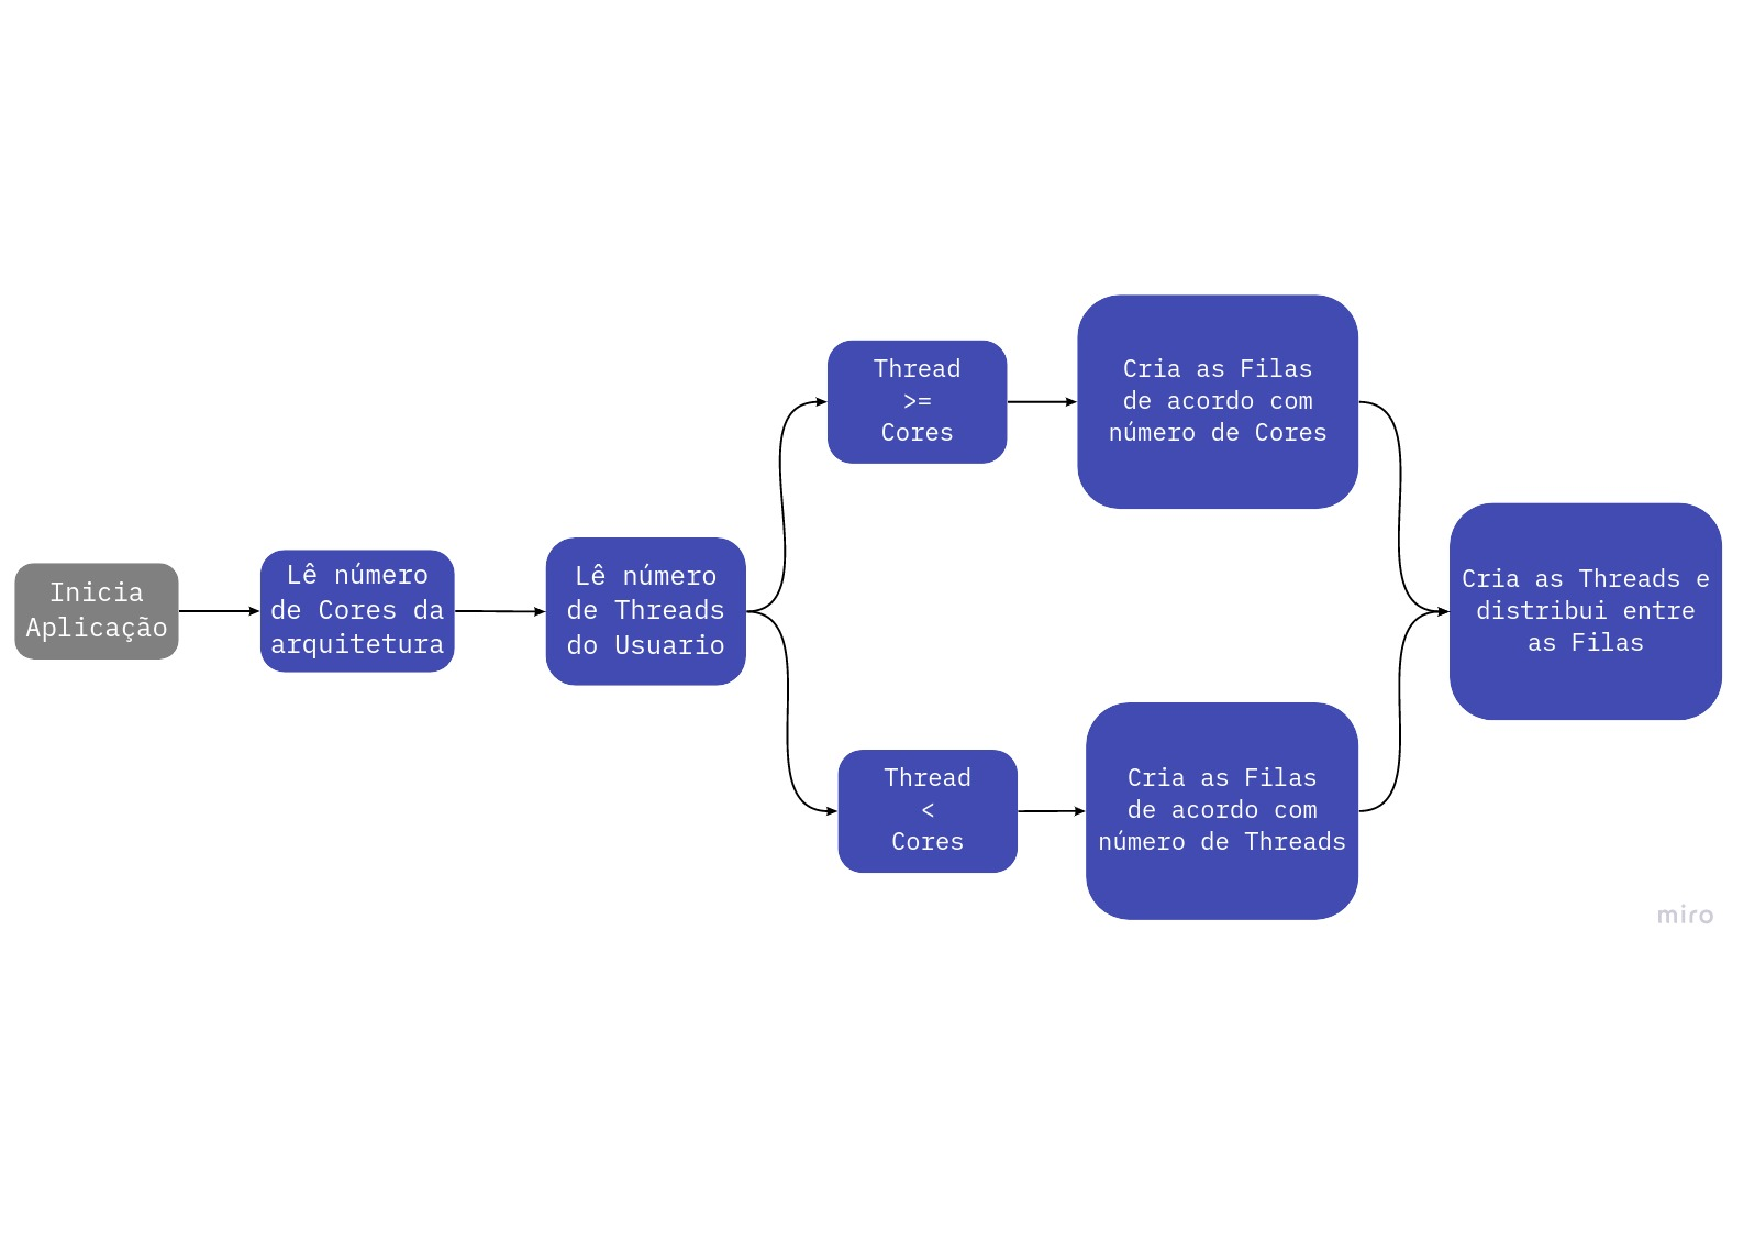
\includegraphics[scale=.5]{images/lstm1}
% \caption{Inicialização da LTMS} 
% \label{LTMS1}
% \end{figure}

% O escalonador foi desenvolvido em C++ para ser utilizado com a biblioteca de STM TinySTM. Para este trabalho foram utilizado os benchmarks do conjunto de benchmark STMAP.

% % Como visto na seção~\ref{section:stamp} o STAMP fornece uma biblioteca de thread chamada thread.h. O LTMS sobrepõem esta biblioteca fornecendo threads no padrão C++ 11 e uma serie de funções de escalonamento e mecanismos de distribuição de tarefas.

% A implementação do LTMS trás um conjunto de funções que utilizam recursos de threads do c++ para executar a aplicação junto com a biblioteca TinySTM. Estes ...

% % Para avaliar a arquitetura e entender o fluxo de execução foram utilizadas dentro do escalonador a biblioteca HwLoc e...

% ...

% \begin{figure}[htbp]
%   \centering 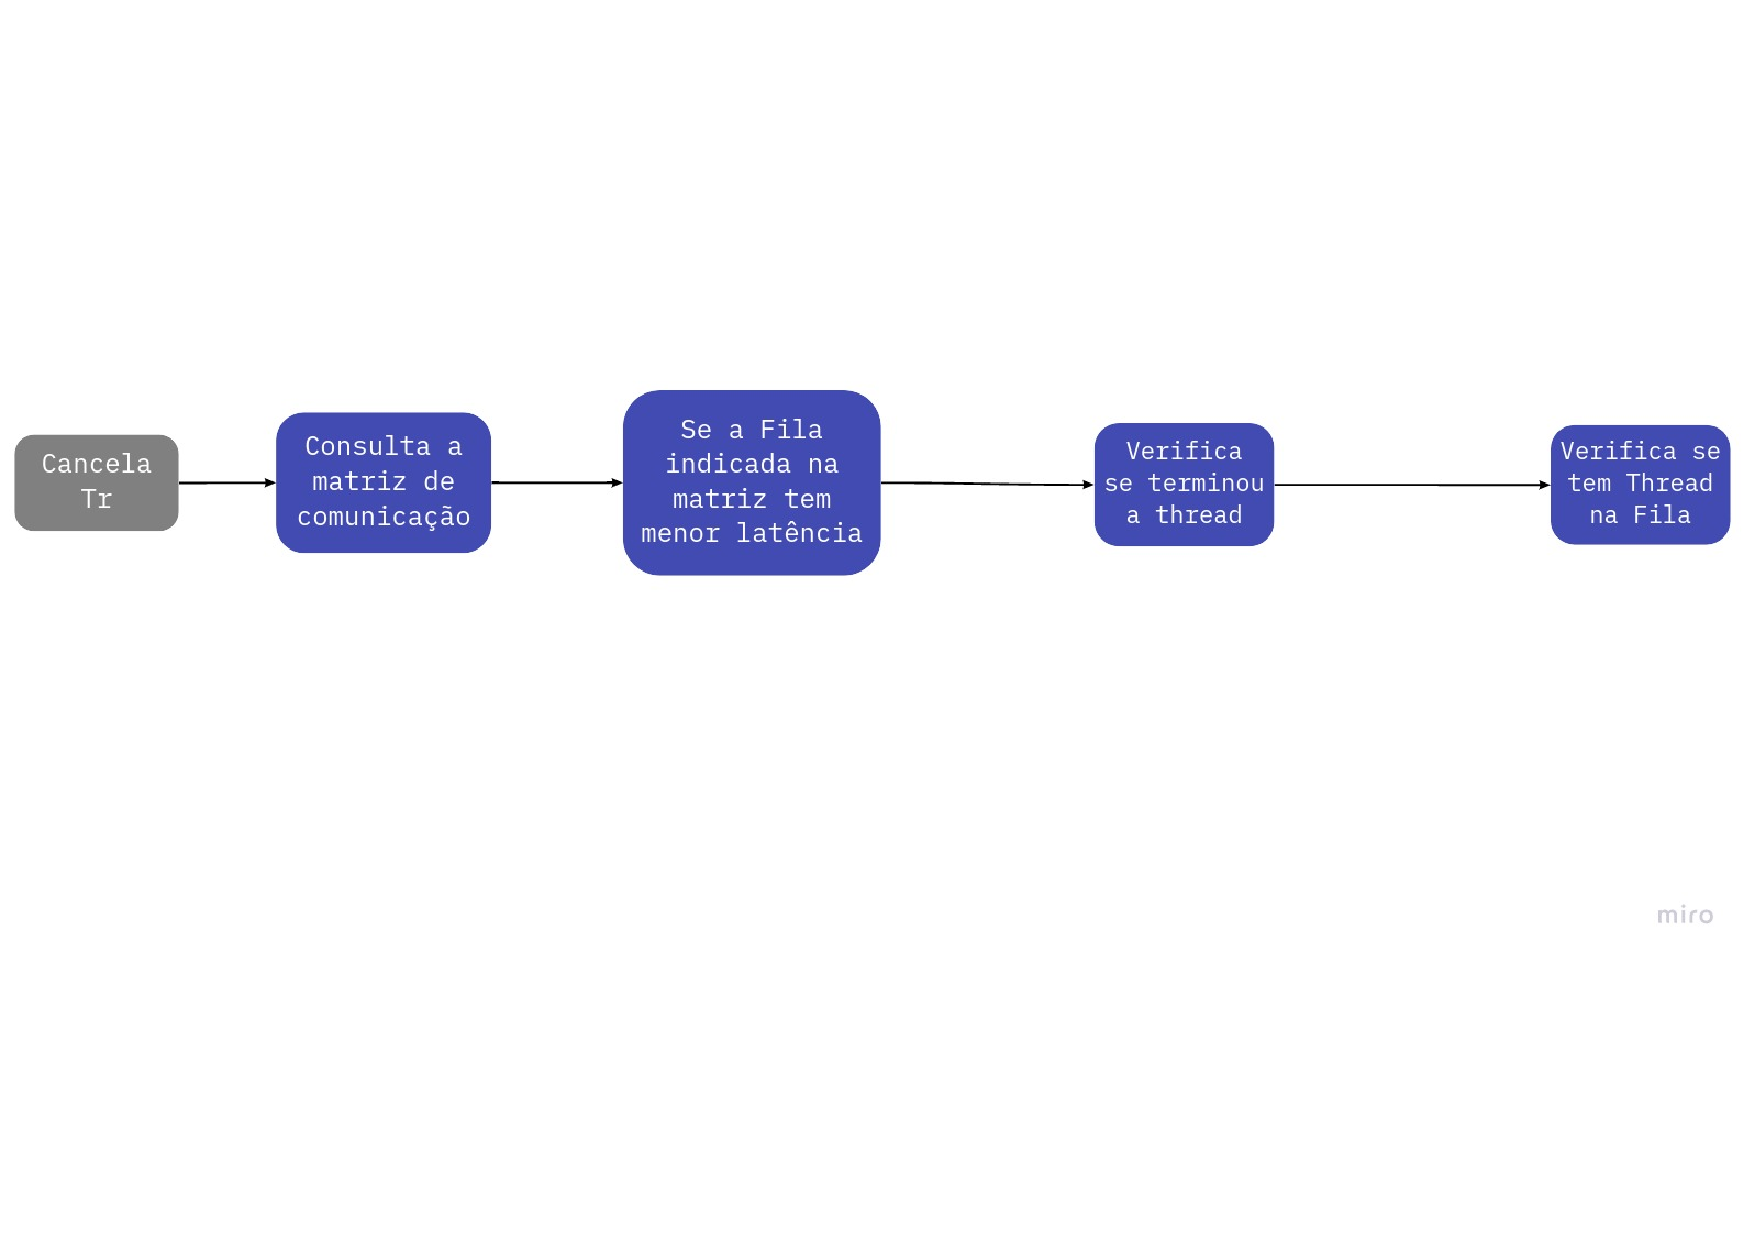
\includegraphics[scale=.5]{images/lstm2}
% \caption{Migração de threads na LTMS} 
% \label{LTMS2}
% \end{figure}

% ...

\chapter{Experimentos}
\label{chapter::experimentos}

% \todo{tem uma seção sobre maquina e uma sobre os parametros?}
Para este trabalho foi desenvolvido um escalonador de STM NUMA-Aware, intitulado LTMS, que funciona em três etapas. Para validação, o escalonador LTMS foi desenvolvido em linguagem C, e aplicado à biblioteca de STM TinySTM em sua versão 1.0.5, e foram rodados experimentos com o conjunto de benchmarks STMAP em sua versão 0.9.10.

% \todo{descrever nós numa... pg112 douglas e característica do xeon}
Os testes foram rodados em uma máquina de arquitetura NUMA com processador Intel Xeon E5-4650 com 96 núcleos e 192 threads em \emph{hyper threading} e 468 Gb de memória RAM, utilizando com sistema operacional Linux Debian kernel 4.19.0-8-amd64  e gcc 8.3.0.

Como comentado anteriormente o LTMS permite que estratégia para distribuição de threads sejam configuradas e heurísticas para migração de threads sejam desenvolvidas e acopladas a ele para avaliar a influencia de diferentes aplicações utilizando o escalonador. Neste trabalho foram desenvolvidas uma estratégia de distribuição com duas configurações e duas heurísticas de migração. Para obter os resultados do LTMS foram rodadas quatro baterias de testes com as seguintes configurações: LTMS com distribuição Sequential e migração Threshold, LTMS com distribuição Sequential e migração Latency, LTMS com distribuição Chunks e migração Threshold, e LTMS com distribuição Chunks e migração Latency. Para comparar o desempenho do escalonador LTMS, foi executada uma bateria de teste com a TinySTM 1.0.5 sem modificações.

% \todo{tabela com os inputs dos benchmarks}
Cada bateria de teste consiste em 30 execuções de cada benchmark do conjunto STAMP, para os cenários de 1, 2, 4, 8, 16, 32, 64, 128, 256, e 512 threads. A seção~\ref{resultados} mostra os resultados obtidos com os experimentos.

\section{Resultados}
\label{resultados}

Para validação deste trabalho foi avaliado o desempenho do LTMS em arquitetura NUMA.  Nestes experimentos utilizamos o processador Intel Xeon E5-4650 com 96 núcleos e 192 threads em \emph{hyper threading}, os experimentos rodaram com cenários de até 512 threads, sendo assim os testes com 256 e 512 threads ultrapassam o limite de threads em \emph{hyper threading} da máquina utilizada.

\subsection{Tempo de execução}

As Figuras abaixo apresentam os resultados com tempo de execução em segundos para os benchmarks testados utilizando todas configurações heurísticas para os cenários de 1 a 512 threads. Temos como base de comparação os resultados obtidos com a TinySTM pura. Para estes experimentos o LTMS apresentou na maioria dos casos um melhor tempo de execução quando comparado a TinySTM. O melhor ganho de desempenho obtido foi para o experimento Intruder de configuração Latency-Sequential com 512 threads que obteve 96\% de redução em seu tempo de execução.

O experimento Bayes~\ref{bayes_tmp} possui um comportamento não determinístico e não é considerado adequado para comparação do tempo de execução~\cite{Ruan:2014}.

\begin{figure}[!ht]
    \centering
    % \subfloat[Bayes]{
        % \label{Bayes}
        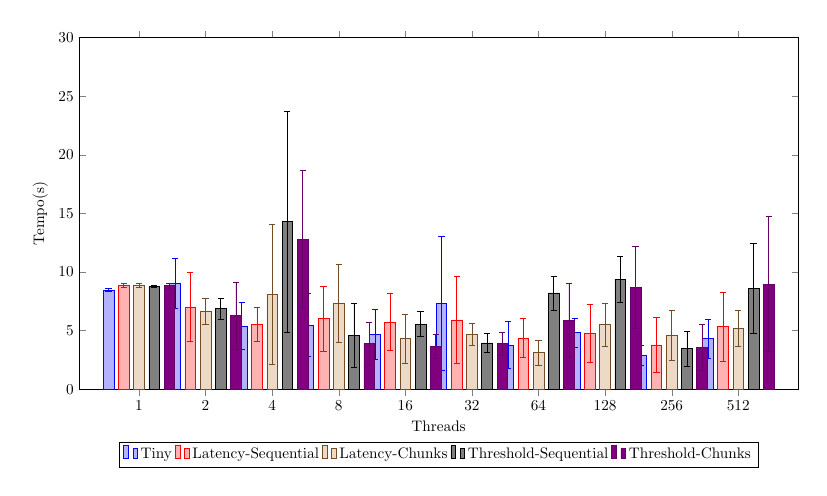
\begin{tikzpicture}[scale=0.55, baseline]
        \begin{axis}[
            width=1.5 \linewidth,
            height=0.8 \linewidth,
            %media de tempo intruder
            ybar=3pt,
            %enlargelimits=0.10,
            legend style={at={(0.5,-0.15)}, anchor=north, legend columns=-1},
            ylabel=Tempo(s),
            xlabel=Threads,
            symbolic x coords={1, 2, 4, 8, 16, 32, 64, 128, 256, 512},
            xtick=data,
            ymin=0,
            ymax=30,
            bar width=7pt,
            % nodes near coords,
            nodes near coords align={vertical},
        ]
        \addplot+[error bars,y dir=both, y explicit] coordinates {
            (1,8.46)+-(1,0.12) (2,9.04)+-(2,2.15) (4,5.41)+-(4,2.01) (8,5.49)+-(8,2.70) (16,4.71)+-(16,2.14) (32,7.33)+-(32,5.74) (64,3.78)+-(64,1.99) (128,4.82)+-(128,1.20) (256,2.87)+-(256,0.84) (512,4.32)+-(512,1.69)
        };
        \addplot+[error bars,y dir=both, y explicit] coordinates {
            (1,8.86)+-(1,0.17) (2,7.02)+-(2,2.95) (4,5.52)+-(4,1.47) (8,6.03)+-(8,2.78) (16,5.75)+-(16,2.44) (32,5.92)+-(32,3.68) (64,4.36)+-(64,1.66) (128,4.78)+-(128,2.50) (256,3.78)+-(256,2.36) (512,5.34)+-(512,2.97)
        };
        \addplot+[error bars,y dir=both, y explicit] coordinates {
            (1,8.87)+-(1,0.14) (2,6.68)+-(2,1.10) (4,8.09)+-(4,5.99) (8,7.33)+-(8,3.29) (16,4.32)+-(16,2.09) (32,4.71)+-(32,0.94) (64,3.12)+-(64,1.09) (128,5.50)+-(128,1.87) (256,4.62)+-(256,2.12) (512,5.18)+-(512,1.52)
        };
        \addplot+[error bars,y dir=both, y explicit] coordinates {
            (1,8.80)+-(1,0.10) (2,6.87)+-(2,0.90) (4,14.29)+-(4,9.42) (8,4.60)+-(8,2.73) (16,5.56)+-(16,1.06) (32,3.95)+-(32,0.79) (64,8.22)+-(64,1.45) (128,9.40)+-(128,1.98) (256,3.48)+-(256,1.49) (512,8.61)+-(512,3.82)
        };
        \addplot+[error bars,y dir=both, y explicit] coordinates {
            (1,8.84)+-(1,0.21) (2,6.29)+-(2,2.84) (4,12.79)+-(4,5.91) (8,3.91)+-(8,1.84) (16,3.66)+-(16,1.03) (32,3.89)+-(32,0.97) (64,5.88)+-(64,3.19) (128,8.70)+-(128,3.51) (256,3.60)+-(256,1.96) (512,8.97)+-(512,5.75)
        };
        \legend {Tiny, Latency-Sequential, Latency-Chunks, Threshold-Sequential, Threshold-Chunks}
        \end{axis}
        \end{tikzpicture}
    % }
    \caption{Tempo de execução em segundos do benchmark Bayes variando o número de \emph{threads}.}
    \label{bayes_tmp}

\end{figure}


% Entretanto este também é apresentado neste trabalho, onde mostra melhor tempo de execução para a TinySTM que o escalonador LTMS na maioria dos cenários de threads. O teste com 4 threads com a configuração Threshold-Sequential apresentou o pior resultado obtendo 164\% de tempo acima da TinySTM. O LTMS também apresentou algumas reduções no tempo de execução quando comparado a TinySTM, o teste Threshold-Chunks obteve uma redução de 46\% no tempo de execução.

No experimento Intruder~\ref{intruder_tmp} o LTMS apresentou melhor tempo de execução para todos os cenários a partir de 2 threads, obtendo uma redução de até 96\% do tempo de execução que ocorreu em Latency-Sequential com 512 threads, e o menor ganho de desempenho foi de 23\% no teste Threshold-Chunks para 4 threads. Todos os resultados do Intruder para uma thread apresentaram maior tempo de execução, obtendo no pior cenário, Threshold-Chunks, um aumento de 24\%.

\begin{figure}[!ht]
    \centering
        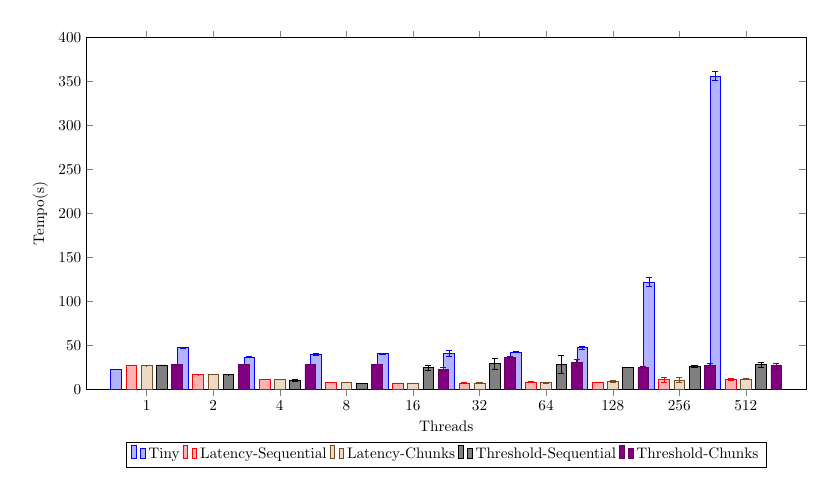
\begin{tikzpicture}[scale=0.55, baseline]
        \begin{axis}[
            width=1.5 \linewidth,
            height=0.8 \linewidth,
            %media de tempo intruder
            ybar=3pt,
            %enlargelimits=0.10,
            legend style={at={(0.5,-0.15)}, anchor=north, legend columns=-1},
            ylabel=Tempo(s),
            xlabel=Threads,
            symbolic x coords={1, 2, 4, 8, 16, 32, 64, 128, 256, 512},
            xtick=data,
            ymin=0,
            ymax=400,
            bar width=7pt,
            % nodes near coords,
            nodes near coords align={vertical},
        ]
        \addplot+[error bars,y dir=both, y explicit] coordinates {
            (1,22.49)+-(1,0.11) (2,47.47)+-(2,0.69) (4,36.62)+-(4,0.59) (8,39.90)+-(8,0.89) (16,40.47)+-(16,0.35) (32,40.54)+-(32,3.55) (64,42.59)+-(64,0.29) (128,47.43)+-(128,1.97) (256,122.18)+-(256,4.64) (512,356.05)+-(512,5.11) 
        };
        \addplot+[error bars,y dir=both, y explicit] coordinates {
            (1,27.06)+-(1,0.18) (2,16.76)+-(2,0.13) (4,11.43)+-(4,0.10) (8,8.18)+-(8,0.13) (16,7.20)+-(16,0.06) (32,7.31)+-(32,0.14) (64,8.25)+-(64,0.81) (128,8.00)+-(128,0.37) (256,10.82)+-(256,3.29) (512,11.20)+-(512,0.86)
        };
        \addplot+[error bars,y dir=both, y explicit] coordinates {
            (1,26.90)+-(1,0.17) (2,16.89)+-(2,0.13) (4,11.50)+-(4,0.13) (8,8.10)+-(8,0.10) (16,7.21)+-(16,0.06) (32,7.28)+-(32,0.07) (64,7.61)+-(64,0.63) (128,9.11)+-(128,0.98) (256,10.40)+-(256,2.68) (512,11.59)+-(512,0.72)
        };
        \addplot+[error bars,y dir=both, y explicit] coordinates {
            (1,27.73)+-(1,0.05) (2,16.65)+-(2,0.16) (4,10.50)+-(4,1.10) (8,6.64)+-(8,0.23) (16,24.42)+-(16,2.56) (32,29.00)+-(32,6.41) (64,28.59)+-(64,10.33) (128,25.01)+-(128,0.29) (256,26.19)+-(256,1.25) (512,27.87)+-(512,2.82)
        };
        \addplot+[error bars,y dir=both, y explicit] coordinates {
            (1,27.96)+-(1,0.25) (2,28.12)+-(2,0.28) (4,28.11)+-(4,0.14) (8,28.17)+-(8,0.07) (16,23.01)+-(16,1.76) (32,36.20)+-(32,1.18) (64,30.24)+-(64,4.39) (128,24.97)+-(128,1.10) (256,26.99)+-(256,2.13) (512,27.18)+-(512,2.84)
        };
        \legend {Tiny, Latency-Sequential, Latency-Chunks, Threshold-Sequential, Threshold-Chunks}
        \end{axis}
        \end{tikzpicture}
    \caption{Tempo de execução em segundos do benchmark Intruder variando o número de \emph{threads}.}
    \label{intruder_tmp}

\end{figure}


O benchmark Kmeans apresenta baixo índice de contenção e gasta pouco tempo dentro das transações~\cite{STAMP}. Este experimento~\ref{kmeans_tempo} apresentou para maioria dos cenários de threads um decremento no tempo de execução do LTMS em relação a TinySTM. O pior resultado ocorreu para o teste Threshold-Chunks com 512 threads e apresentou um aumento de 45\% no tempo de execução, e o melhor resultado ocorreu para o teste Threshold-Sequential com 8 threads e apresentou um decremento de 80\% no tempo de execução.

\begin{figure}[!ht]
    \centering
        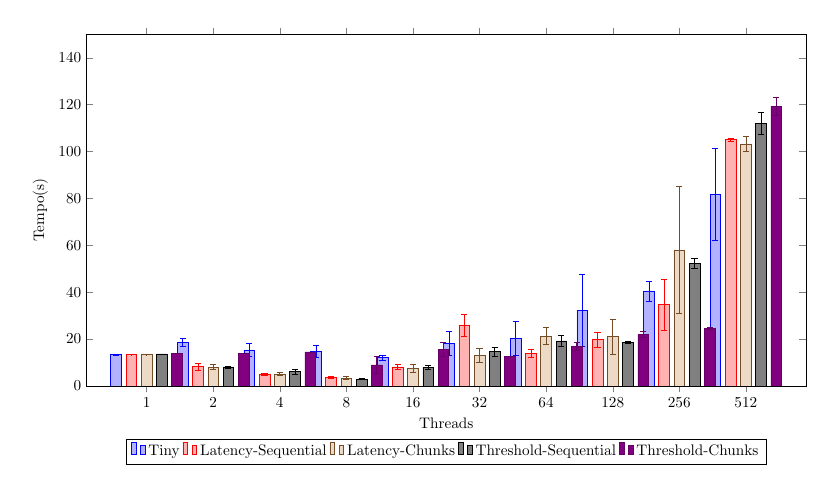
\begin{tikzpicture}[scale=0.55, baseline]
        \begin{axis}[
            width=1.5 \linewidth,
            height=0.8 \linewidth,
            %media de tempo intruder
            ybar=3pt,
            %enlargelimits=0.10,
            legend style={at={(0.5,-0.15)}, anchor=north, legend columns=-1},
            ylabel=Tempo(s),
            xlabel=Threads,
            symbolic x coords={1, 2, 4, 8, 16, 32, 64, 128, 256, 512},
            xtick=data,
            ymin=0,
            ymax=150,
            bar width=7pt,
            % nodes near coords,
            nodes near coords align={vertical},
        ]
        \addplot+[error bars,y dir=both, y explicit] coordinates {
            (1,13.32)+-(1,0.05) (2,18.64)+-(2,1.86) (4,15.33)+-(4,2.68) (8,14.72)+-(8,2.44) (16,12.06)+-(16,0.95) (32,18.24)+-(32,5.19) (64,20.20)+-(64,7.21) (128,32.16)+-(128,15.30) (256,40.54)+-(256,4.28) (512,81.86)+-(512,19.67) 
        };
        \addplot+[error bars,y dir=both, y explicit] coordinates {
            (1,13.36)+-(1,0.05) (2,8.25)+-(2,1.41) (4,5.05)+-(4,0.53) (8,3.49)+-(8,0.45) (16,8.10)+-(16,1.15) (32,25.81)+-(32,4.77) (64,14.01)+-(64,1.61) (128,19.77)+-(128,3.11) (256,34.76)+-(256,10.90) (512,105.07)+-(512,0.66)
        };
        \addplot+[error bars,y dir=both, y explicit] coordinates {
            (1,13.39)+-(1,0.03) (2,8.05)+-(2,1.09) (4,5.13)+-(4,0.64) (8,3.37)+-(8,0.57) (16,7.62)+-(16,1.79) (32,13.01)+-(32,3.05) (64,21.35)+-(64,3.62) (128,21.05)+-(128,7.45) (256,57.98)+-(256,27.06) (512,103.22)+-(512,3.24)
        };
        \addplot+[error bars,y dir=both, y explicit] coordinates {
            (1,13.70)+-(1,0.00) (2,8.08)+-(2,0.39) (4,6.03)+-(4,1.01) (8,2.85)+-(8,0.20) (16,7.92)+-(16,1.01) (32,14.57)+-(32,1.81) (64,19.24)+-(64,2.21) (128,18.49)+-(128,0.48) (256,52.31)+-(256,2.27) (512,111.88)+-(512,4.66) 
        };
        \addplot+[error bars,y dir=both, y explicit] coordinates {
            (1,13.73)+-(1,0.00) (2,13.72)+-(2,0.00) (4,14.49)+-(4,0.02) (8,8.98)+-(8,3.78) (16,15.66)+-(16,2.82) (32,12.59)+-(32,0.01) (64,16.86)+-(64,1.83) (128,21.99)+-(128,1.45) (256,24.41)+-(256,0.44) (512,119.27)+-(512,3.89)
        };
        \legend {Tiny, Latency-Sequential, Latency-Chunks, Threshold-Sequential, Threshold-Chunks}
        \end{axis}
        \end{tikzpicture}
    
    \caption{Tempo de execução em segundos do benchmark Kmeans variando o número de \emph{threads}.}
    \label{kmeans_tempo}

\end{figure}


No experimento Labyrinth~\ref{labyrinth_tempo} o LTMS apresentou para maioria dos cenários um decremento no tempo de execução. O melhor tempo de execução em relação a TinySTM pode ser observado no teste Latency-Sequential para 512 threads, onde é observado uma redução de 54\% do tempo de execução. O pior cenário para o LTMS apresenta um aumento de 29\% que foi observado no teste Latency-Chunks 16 threads. Esta aplicação possui alta contenção e o tempo dentro da transação é longo. O Labyrinth também possui como característica o acesso a um grande número de endereços distintos.

\begin{figure}[!ht]
    \centering
        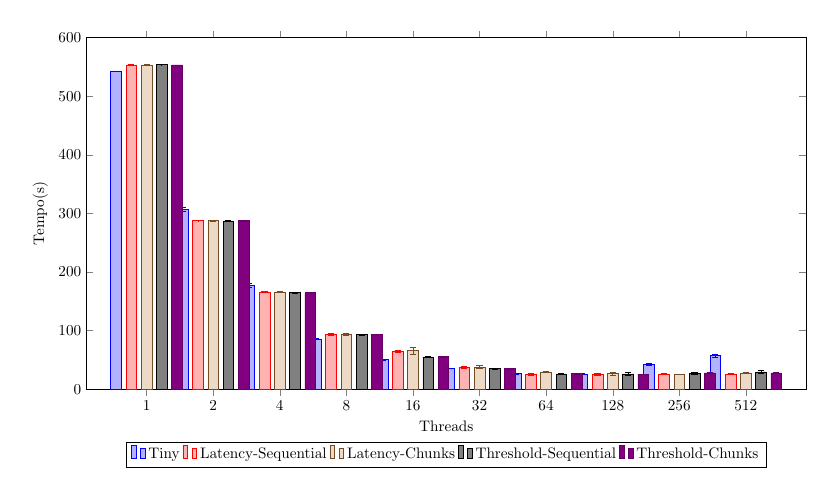
\begin{tikzpicture}[scale=0.55, baseline]
            \begin{axis}[
                width=1.5 \linewidth,
                height=0.8 \linewidth,
                %media de tempo intruder
                ybar=3pt,
                %enlargelimits=0.10,
                legend style={at={(0.5,-0.15)}, anchor=north, legend columns=-1},
                ylabel=Tempo(s),
            xlabel=Threads,
                symbolic x coords={1, 2, 4, 8, 16, 32, 64, 128, 256, 512},
                xtick=data,
                ymin=0,
                ymax=600,
                bar width=7pt,
                % nodes near coords,
                nodes near coords align={vertical},
            ]
            \addplot+[error bars,y dir=both, y explicit] coordinates {
                (1,543.12)+-(1,0.14) (2,307.12)+-(2,3.77) (4,177.18)+-(4,3.79) (8,86.06)+-(8,0.82) (16,50.63)+-(16,0.60) (32,35.89)+-(32,0.53) (64,26.45)+-(64,0.63) (128,25.83)+-(128,0.64) (256,41.98)+-(256,1.85) (512,57.32)+-(512,2.08) 
            };
            \addplot+[error bars,y dir=both, y explicit] coordinates {
                (1,553.57)+-(1,0.26) (2,287.70)+-(2,0.17) (4,165.86)+-(4,0.67) (8,94.13)+-(8,1.50) (16,65.04)+-(16,2.20) (32,37.22)+-(32,1.17) (64,25.60)+-(64,1.00) (128,25.49)+-(128,1.49) (256,26.10)+-(256,1.15) (512,25.80)+-(512,0.75)
            };
            \addplot+[error bars,y dir=both, y explicit] coordinates {
                (1,553.49)+-(1,0.21)(2,287.57)+-(2,0.25)(4,165.74)+-(4,0.99)(8,93.35)+-(8,1.29)(16,65.67)+-(16,6.11)(32,38.25)+-(32,1.76)(64,29.61)+-(64,0.77)(128,26.85)+-(128,2.24)(256,25.63)+-(256,0.42)(512,27.96)+-(512,1.35)
            };
            \addplot+[error bars,y dir=both, y explicit] coordinates {
                (1,553.89)+-(1,0.08) (2,287.30)+-(2,0.32) (4,164.88)+-(4,0.69) (8,93.33)+-(8,0.76) (16,55.06)+-(16,0.46) (32,35.27)+-(32,0.97) (64,26.35)+-(64,1.17) (128,26.33)+-(128,1.74) (256,26.96)+-(256,1.43) (512,29.70)+-(512,2.27) 
            };
            \addplot+[error bars,y dir=both, y explicit] coordinates {
                (1,553.38)+-(1,0.02) (2,287.58)+-(2,0.22) (4,164.99)+-(4,0.38) (8,93.83)+-(8,0.15) (16,55.92)+-(16,0.76) (32,35.17)+-(32,0.71) (64,26.79)+-(64,0.74) (128,25.67)+-(128,0.66) (256,27.99)+-(256,1.60) (512,28.01)+-(512,0.74)
            };
        \legend {Tiny, Latency-Sequential, Latency-Chunks, Threshold-Sequential, Threshold-Chunks}
        \end{axis}
        \end{tikzpicture}
    \caption{Tempo de execução em segundos do benchmark Labyrinth variando o número de \emph{threads}.}
    \label{labyrinth_tempo}

\end{figure}


No experimento Vacation~\ref{vacation_tempo} foi observado uma redução de 81\% do tempo de execução para o teste Latency-Sequential com 512 threads, a maioria dos cenários de threads do Vacation apresentam uma redução no tempo de execução do LTMS quando comparados ao TinySTM, porém, alguns cenários apresentaram um aumento no tempo de execução, o pior cenário possui um aumento de 64\% do tempo e pode ser visualizado no teste Latency-Chunks com 128 threads. Esta aplicação possui contenção média e o tempo dentro da transação é longo.

\begin{figure}[!ht]
    \centering
        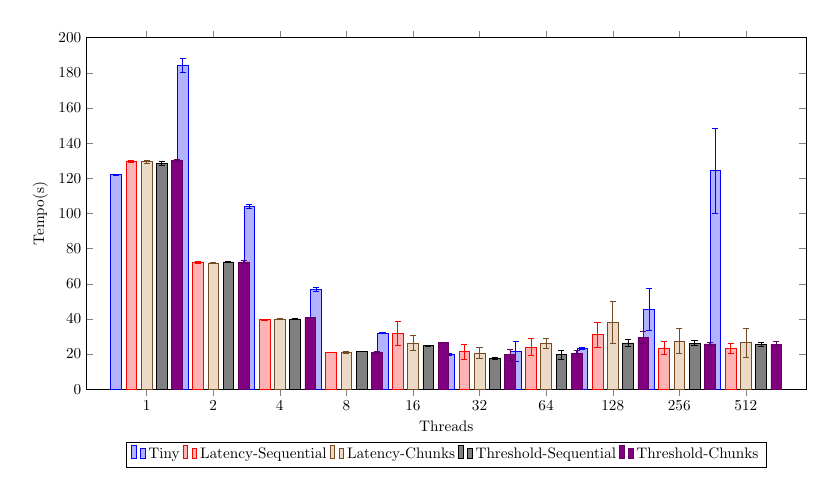
\begin{tikzpicture}[scale=0.55, baseline]
        \begin{axis}[
            width=1.5 \linewidth,
            height=0.8 \linewidth,
            %media de tempo intruder
            ybar=3pt,
            %enlargelimits=0.10,
            legend style={at={(0.5,-0.15)}, anchor=north, legend columns=-1},
            ylabel=Tempo(s),
            xlabel=Threads,
            symbolic x coords={1, 2, 4, 8, 16, 32, 64, 128, 256, 512},
            xtick=data,
            ymin=0,
            ymax=200,
            bar width=7pt,
            % nodes near coords,
            nodes near coords align={vertical},
        ]
        \addplot+[error bars,y dir=both, y explicit] coordinates {
            (1,122.19)+-(1,0.35) (2,184.47)+-(2,3.93) (4,103.92)+-(4,1.04) (8,56.80)+-(8,1.07) (16,31.99)+-(16,0.24) (32,19.69)+-(32,0.52) (64,21.68)+-(64,5.72) (128,23.22)+-(128,0.57) (256,45.58)+-(256,11.99) (512,124.45)+-(512,24.20) 
        };
        \addplot+[error bars,y dir=both, y explicit] coordinates {
            (1,129.87)+-(1,0.52) (2,72.20)+-(2,0.44) (4,39.59)+-(4,0.19) (8,21.14)+-(8,0.09) (16,31.78)+-(16,6.87) (32,21.39)+-(32,4.41) (64,24.02)+-(64,4.93) (128,31.01)+-(128,7.24) (256,23.53)+-(256,3.50) (512,23.21)+-(512,3.03)
        };
        \addplot+[error bars,y dir=both, y explicit] coordinates {
            (1,129.58)+-(1,0.88) (2,71.87)+-(2,0.48) (4,39.90)+-(4,0.39) (8,21.15)+-(8,0.64) (16,26.35)+-(16,4.18) (32,20.69)+-(32,3.15) (64,26.17)+-(64,3.04) (128,38.12)+-(128,12.03) (256,27.50)+-(256,7.32) (512,26.48)+-(512,8.21)
        };
        \addplot+[error bars,y dir=both, y explicit] coordinates {
            (1,128.56)+-(1,0.95) (2,72.45)+-(2,0.41) (4,40.00)+-(4,0.22) (8,21.55)+-(8,0.22) (16,24.76)+-(16,0.20) (32,17.51)+-(32,0.39) (64,19.62)+-(64,2.71) (128,26.34)+-(128,1.81) (256,26.30)+-(256,1.52) (512,25.59)+-(512,1.05) 
        };
        \addplot+[error bars,y dir=both, y explicit] coordinates {
            (1,130.29)+-(1,0.63) (2,72.49)+-(2,0.59) (4,40.83)+-(4,0.31) (8,21.11)+-(8,0.63) (16,26.56)+-(16,0.15) (32,19.76)+-(32,3.23) (64,20.45)+-(64,1.74) (128,29.49)+-(128,3.46) (256,25.76)+-(256,0.95) (512,25.70)+-(512,1.49)
        };
    \legend {Tiny, Latency-Sequential, Latency-Chunks, Threshold-Sequential, Threshold-Chunks}
        \end{axis}
        \end{tikzpicture}
    \caption{Tempo de execução em segundos do benchmark Vacation variando o número de \emph{threads}.}
    \label{vacation_tempo}

\end{figure}


O benchmark Yada~\ref{yada_tempo} possui contenção média e o tempo dentro da transação é longo. Outra característica do benchmark está em seu acesso a uma quantidade média de endereços distintos. O experimento também apresentou para a maioria dos testes uma redução do tempo de execução do LTMS em comparação a TinySTM. O LTMS obteve uma redução de até 92\% do tempo de execução para o teste Latency-Chunks com 512 threads. O benchmark também apresentou uma redução do tempo de execução de 70\% para o teste Threshold-Chunks com 16 threads.

\begin{figure}[!ht]
    \centering
        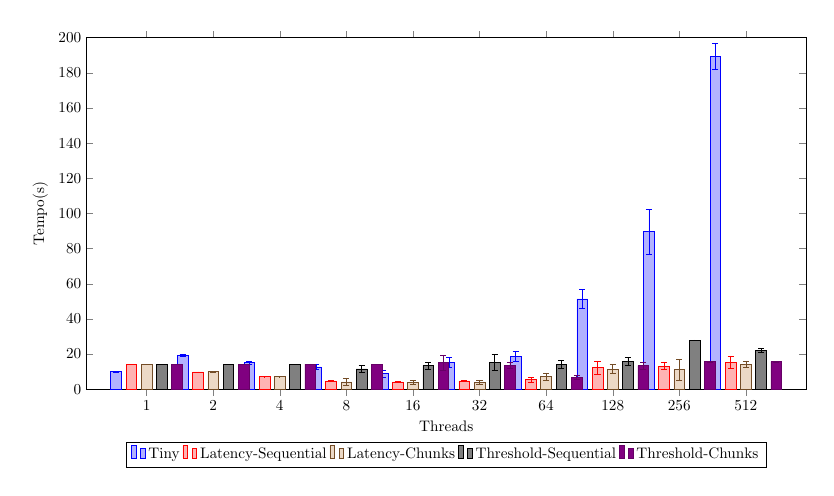
\begin{tikzpicture}[scale=0.55, baseline]
        \begin{axis}[
            width=1.5 \linewidth,
            height=0.8 \linewidth,
            %media de tempo intruder
            ybar=3pt,
            %enlargelimits=0.10,
            legend style={at={(0.5,-0.15)}, anchor=north, legend columns=-1},
            ylabel=Tempo(s),
            xlabel=Threads,
            symbolic x coords={1, 2, 4, 8, 16, 32, 64, 128, 256, 512},
            xtick=data,
            ymin=0,
            ymax=200,
            bar width=7pt,
            % nodes near coords,
            nodes near coords align={vertical},
        ]
        \addplot+[error bars,y dir=both, y explicit] coordinates {
            (1,9.95)+-(1,0.09) (2,19.42)+-(2,0.50) (4,15.05)+-(4,1.07) (8,12.75)+-(8,1.30) (16,8.85)+-(16,1.90) (32,15.25)+-(32,2.69) (64,18.85)+-(64,2.74) (128,51.34)+-(128,5.50) (256,89.66)+-(256,12.90) (512,189.43)+-(512,7.63) 
        };
        \addplot+[error bars,y dir=both, y explicit] coordinates {
            (1,14.09)+-(1,0.09) (2,9.88)+-(2,0.04) (4,7.22)+-(4,0.04) (8,4.78)+-(8,0.29) (16,4.19)+-(16,0.35) (32,4.74)+-(32,0.50) (64,5.38)+-(64,1.21) (128,12.38)+-(128,3.72) (256,13.14)+-(256,2.01) (512,15.43)+-(512,3.54)
        };
        \addplot+[error bars,y dir=both, y explicit] coordinates {
            (1,14.31)+-(1,0.16) (2,9.98)+-(2,0.07) (4,7.23)+-(4,0.11) (8,4.19)+-(8,1.93) (16,3.85)+-(16,0.97) (32,3.96)+-(32,1.37) (64,7.11)+-(64,1.83) (128,11.47)+-(128,2.48) (256,11.12)+-(256,5.94) (512,14.17)+-(512,1.47)
        };
        \addplot+[error bars,y dir=both, y explicit] coordinates {
            (1,14.17)+-(1,0.05) (2,14.17)+-(2,0.11) (4,14.20)+-(4,0.08) (8,11.61)+-(8,2.13) (16,13.53)+-(16,1.93) (32,15.15)+-(32,4.48) (64,14.19)+-(64,2.00) (128,15.69)+-(128,2.21) (256,27.92)+-(256,0.20) (512,22.18)+-(512,1.28) 
        };
        \addplot+[error bars,y dir=both, y explicit] coordinates {
            (1,14.35)+-(1,0.05) (2,14.29)+-(2,0.04) (4,14.31)+-(4,0.08) (8,14.31)+-(8,0.05) (16,15.07)+-(16,4.06) (32,13.64)+-(32,1.83) (64,6.83)+-(64,1.09) (128,13.37)+-(128,2.19) (256,15.65)+-(256,0.16) (512,15.73)+-(512,0.14)
        };
        \legend {Tiny, Latency-Sequential, Latency-Chunks, Threshold-Sequential, Threshold-Chunks}
        \end{axis}
        \end{tikzpicture}
    \caption{Tempo de execução em segundos do benchmark Yada variando o número de \emph{threads}.}
    \label{yada_tempo}

\end{figure}


Os resultados apresentam para maioria dos benchmarks um resultado melhor de desempenho utilizando o escalonador proposto neste trabalho. Quando ultrapassado o número de threads hyper threading disponíveis na arquitetura utilizada, os únicos benchmarks que não obtiveram resultados de tempo abaixo da TinySTM foram os benchmarks Bayes e Kmeans. Para o benchmark Bayes, a sua ordem de commits no início da execução afeta seu tempo de execução final~\cite{Ruan:2014}, o que torna seu comportamento não determinístico e dificulta a sua avaliação.

O benchmark Kmeans, possui baixa contenção e um tempo baixo de execução das transações, este benchmark também tem como característica o acesso a uma pequena quantidade de endereços distintos. Estas características contribuíram para que o escalonador obteve-se uma redução no tempo de execução até 128 threads, o que fica dentro da quantidade de threads disponível pela arquitetura utilizada. Porém, acima com 256 threads o escalonador apresentou tempo de execução acima da TinySTM em alguns cenários.

Os demais benchmarks apresentam uma redução significativa em seu tempo de execução para todos cenários de threads, sendo que demonstram maior expressividade para os cenários acima de 256 threads, aqui representando o cenário superior as threads disponíveis na arquitetura.

\subsection{Aborts}

As figuras abaixo apresentam os resultados de quantidades de aborts obtidos nos experimentos descritos neste capítulo, estes gráficos estão em escala logarítmica. Tendo como base de comparação a biblioteca TinySTM, o LTMS apresentou para maioria dos benchmarks um resultado superior, reduzindo no melhor caso até 99\% do número de aborts existentes nas aplicações, esse resultado pode ser observado nos benchmarks Intruder, Kmeans, Vacation e Yada. Os benchmarks Intruder e Yada utilizando Latency-Sequential para 512 threads apresentaram ganho de 99,99\% na redução de aborts. Os benchmarks Kmeans utilizando Threshold-Sequential e Vacations utilizando Latency-Chunks reduziram respectivamente 99,88\% e 99,84\% dos aborts para o cenário de 512 threads.

% O experimento Bayes~\ref{abortBayes} com o LTMS apresenta para maioria dos testes um aumento no número de aborts. O teste Latency-Chunks com 4 threads apresentou um aumento de 18\% no número de aborts. Por outro lado, o escalonador obteve para Latency-Sequential com 2 threads uma redução de 34\% na média dos aborts.

No experimento Intruder~\ref{intruder_abort} foi obtido ganho de desempenho para todos cenários de threads e configurações do escalonador. O melhor resultado pode ser observado para Latency-Sequential com 512 threads, no qual foi obtido 99\% de redução nos aborts. A menor redução nos aborts ocorreu para Threshold-Sequential com 2 threads, onde foi observado a redução de 89\% dos aborts.

\begin{figure}[!ht]
    \centering
        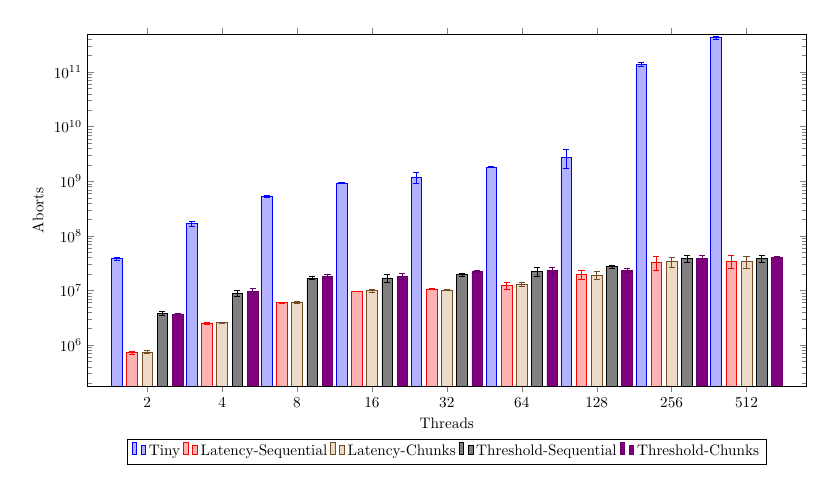
\begin{tikzpicture}[scale=0.55, baseline]
        \begin{axis}[
            ymode=log,
            width=1.5 \linewidth,
            height=0.8 \linewidth,
            %media de tempo intruder
            ybar=3pt,
            %enlargelimits=0.10,
            legend style={at={(0.5,-0.15)}, anchor=north, legend columns=-1},
            ylabel=Aborts,
            xlabel=Threads,
            symbolic x coords={1, 2, 4, 8, 16, 32, 64, 128, 256, 512},
            xtick=data,
            ymin=0,
            ymax=490000000000,
            bar width=7pt,
            % nodes near coords,
            nodes near coords align={vertical},
        ]
        \addplot+[error bars,y dir=both, y explicit] coordinates {
            (1,0.0)+-(1,0.0) (2,38000260.8)+-(2,2949711.678076852) (4,166325696.4)+-(4,18557044.648063533) (8,529197870.6)+-(8,22132676.255908735) (16,924927047.6)+-(16,24358107.18760883) (32,1183579117.4)+-(32,270222169.9344623) (64,1831169740.8)+-(64,62890886.257802844) (128,2763435636.6)+-(128,1003746150.3805901) (256,138779112147.6)+-(256,10430244205.851603) (512,431443096033.6)+-(512,28705521954.994297) 
        };
        \addplot+[error bars,y dir=both, y explicit] coordinates {
            (1,0.0)+-(1,0.0) (2,724967.4)+-(2,38086.07014959669) (4,2505616.2)+-(4,79429.60770745378) (8,6012716.4)+-(8,169677.49348290125) (16,9639253.0)+-(16,142573.7883104745) (32,10568731.0)+-(32,292443.9680909832) (64,12171771.4)+-(64,1784435.4526392485) (128,19342142.8)+-(128,3669581.5184994815) (256,32980054.25)+-(256,9356623.644361822) (512,34119006.5)+-(512,8983159.5)
        };
        \addplot+[error bars,y dir=both, y explicit] coordinates {
             (1,0.0)+-(1,0.0) (2,745630.2)+-(2,40338.85590792084) (4,2559770.6)+-(4,81679.883166175) (8,6127472.777777778)+-(8,267489.386445634) (16,9889825.3)+-(16,755124.9867329315) (32,10236117.3)+-(32,288410.38292407227) (64,13078693.1)+-(64,982436.3361754746) (128,19063545.666666668)+-(128,2925827.5185046173) (256,33704832.6)+-(256,6772680.448815952) (512,34183921.0)+-(512,8274893.22) 
        };
        \addplot+[error bars,y dir=both, y explicit] coordinates {
            (1,0.0)+-(1,0.0) (2,3808172.2)+-(2,327085.8815720422) (4,9023407.8)+-(4,1123234.4180183227) (8,16872564.2)+-(8,1114383.5354166715) (16,17004377.2)+-(16,2666034.739783216) (32,19648666.0)+-(32,1287522.1930899676) (64,22307089.8)+-(64,4029768.617032169) (128,27162139.0)+-(128,1504557.0) (256,38132893.15)+-(256,4958389.304) (512,37984673.0)+-(512,5282793.33)
        };
        \addplot+[error bars,y dir=both, y explicit] coordinates {
            (1,0.0)+-(1,0.0) (2,3578932.78)+-(2,176854.86) (4,9738434.34)+-(4,1124342.85) (8,17928374.6)+-(8,1573847.9) (16,18301736.6)+-(16,2468736.987185277) (32,22436982.0)+-(32,1106602.0) (64,23420167.2)+-(64,3281430.727250502) (128,23366253.0)+-(128,1919489.0) (256,38736187.88)+-(256,5748878.34) (512,39763372.723)+-(512,3174827.12)
        };
        \legend {Tiny, Latency-Sequential, Latency-Chunks, Threshold-Sequential, Threshold-Chunks}
        \end{axis}
        \end{tikzpicture}
    \caption{Aborts do benchmark Intruder variando o número de \emph{threads}.}
    \label{intruder_abort}
\end{figure}


O experimento Kmeans~\ref{kmeans_abort} assim como Intruder, apresenta redução do número de aborts para todos os cenários e configurações. Podemos observar uma redução de até 99\% para Threshold-Sequential com 512 threads. O pior caso do benchmark Kmeans apresentou uma redução de 71\% dos aborts e pode ser observado no Latency-Sequential com 32 threads.

\begin{figure}[!ht]
    \centering
        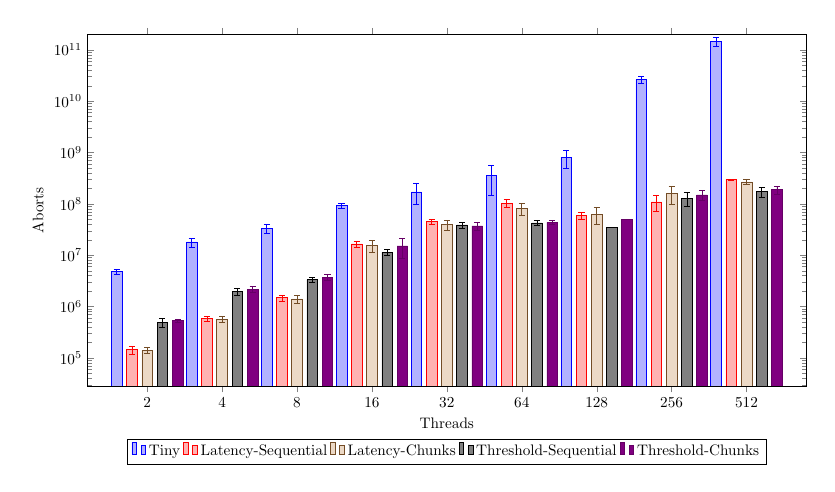
\begin{tikzpicture}[scale=0.55, baseline]
        \begin{axis}[
            ymode=log,
            width=1.5 \linewidth,
            height=0.8 \linewidth,
            %media de tempo intruder
            ybar=3pt,
            %enlargelimits=0.10,
            legend style={at={(0.5,-0.15)}, anchor=north, legend columns=-1},
            ylabel=Aborts,
            xlabel=Threads,
            symbolic x coords={1, 2, 4, 8, 16, 32, 64, 128, 256, 512},
            xtick=data,
            ymin=0,
            ymax=200000000000,
            bar width=7pt,
            % nodes near coords,
            nodes near coords align={vertical},
        ]
        \addplot+[error bars,y dir=both, y explicit] coordinates {
            (1,0.0)+-(1,0.0) (2,4797421.2)+-(2,479774.7418784778) (4,18101846.8)+-(4,3591708.3539415835) (8,33182746.2)+-(8,6732288.556793311) (16,93057923.8)+-(16,9863144.322012922) (32,171442797.6)+-(32,74829388.10384364) (64,359745893.2)+-(64,213043475.04545623) (128,807753260.2)+-(128,310719932.9857997) (256,26569175006.4)+-(256,4470117158.120106) (512,146296330743.6)+-(512,26886172215.929005) 
        };
        \addplot+[error bars,y dir=both, y explicit] coordinates {
            (1,0.0)+-(1,0.0) (2,144295.6)+-(2,24864.282793597726) (4,579330.6)+-(4,68221.2484981036) (8,1486520.2)+-(8,200173.524986098) (16,16580311.4)+-(16,2227873.6890443857) (32,45063610.6)+-(32,5053643.0020858655) (64,103498202.6)+-(64,18052939.09375) (128,59441333.6)+-(128,8917614.717479235) (256,109146323.8)+-(256,36880499.382352196) (512,294773353.4)+-(512,3281309.7536428105)
        };
        \addplot+[error bars,y dir=both, y explicit] coordinates {
             (1,0.0)+-(1,0.0) (2,141609.1)+-(2,19957.913370139675) (4,570320.1)+-(4,69142.6626511447) (8,1412101.5)+-(8,239771.55806068826) (16,15454899.8)+-(16,3814349.1856658272) (32,39591108.222222224)+-(32,9286948.71968007) (64,81659510.1)+-(64,21584431.489666473) (128,62701912.9)+-(128,22625798.149042867) (256,157892521.1)+-(256,60541141.358650364) (512,267641468.75)+-(512,32356420.707834) 
        };
        \addplot+[error bars,y dir=both, y explicit] coordinates {
            (1,0.0)+-(1,0.0) (2,489474.6)+-(2,95557.56667391652) (4,1982817.6)+-(4,324496.7328282983) (8,3338695.4)+-(8,339537.1836017964) (16,11407592.4)+-(16,1467579.9615602007) (32,38923440.666666664)+-(32,5311247.22872386) (64,42424191.0)+-(64,4907763.0) (128,34826711.0)+-(128,578473.0) (256,128783746.63)+-(256,37482783.86) (512,173847878.28)+-(512,37384778.0)
        };
        \addplot+[error bars,y dir=both, y explicit] coordinates {
            (1,0.0)+-(1,0.0) (2,528574.7)+-(2,29384.0) (4,2157923.0)+-(4,283746.0) (8,3736425.62)+-(8,429388.0) (16,15208687.0)+-(16,6397145.233711557) (32,37279545.0)+-(32,6425946.0) (64,43456253.0)+-(64,3849829.0) (128,49875516.0)+-(128,675193.0) (256,148983127.32)+-(256,31827833.0) (512,187678278.0)+-(512,32738943.73)
        };
        \legend {Tiny, Latency-Sequential, Latency-Chunks, Threshold-Sequential, Threshold-Chunks}
        \end{axis}
        \end{tikzpicture}
    \caption{Aborts do benchmark Kmeans variando o número de \emph{threads}.}
    \label{kmeans_abort}

\end{figure}


No experimento Labyrinth~\ref{labyrinth_abort} apresentou para maioria dos cenários um decremento do número de aborts. O LTMS obteve até 54\% de redução dos aborts, este resultado foi obtido no experimento Latency-Chunks com 512 threads. O LTMS também obteve um aumento de 12\% dos aborts em relação a TinySTM para o teste Threshold-Chunks com 16 threads.

\begin{figure}[!ht]
    \centering
        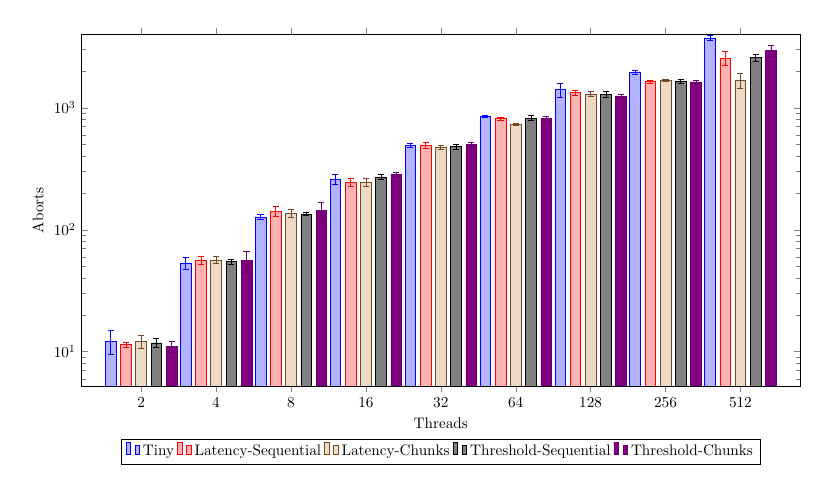
\begin{tikzpicture}[scale=0.55, baseline]
        \begin{axis}[
            ymode=log,
            width=1.5 \linewidth,
            height=0.8 \linewidth,
            %media de tempo intruder
            ybar=3pt,
            %enlargelimits=0.10,
            legend style={at={(0.5,-0.15)}, anchor=north, legend columns=-1},
            ylabel=Aborts,
            xlabel=Threads,
            symbolic x coords={1, 2, 4, 8, 16, 32, 64, 128, 256, 512},
            xtick=data,
            ymin=0,
            ymax=4000,
            bar width=7pt,
            % nodes near coords,
            nodes near coords align={vertical},
        ]
        \addplot+[error bars,y dir=both, y explicit] coordinates {
            (1,0.0)+-(1,0.0) (2,12.2)+-(2,2.63) (4,53.2)+-(4,5.94) (8,127.2)+-(8,6.14) (16,258.0)+-(16,24.04) (32,490.2)+-(32,16.41) (64,847.0)+-(64,12.39) (128,1413.4)+-(128,186.85) (256,1959.6)+-(256,67.08) (512,3727.2)+-(512,167.11) 
        };
        \addplot+[error bars,y dir=both, y explicit] coordinates {
            (1,0.0)+-(1,0.0) (2,11.4)+-(2,0.48) (4,56.0)+-(4,4.09) (8,142.0)+-(8,12.85) (16,245.8)+-(16,19.87) (32,491.2)+-(32,25.11) (64,811.8)+-(64,28.18) (128,1334.2)+-(128,63.09) (256,1633.4)+-(256,41.57) (512,2556.6)+-(512,340.72)
        };
        \addplot+[error bars,y dir=both, y explicit] coordinates {
             (1,0.0)+-(1,0.0) (2,12.2)+-(2,1.46) (4,56.4)+-(4,3.61) (8,136.4)+-(8,10.30) (16,245.4)+-(16,19.39) (32,473.2)+-(32,16.47) (64,734.8)+-(64,11.12) (128,1298.4)+-(128,60.09) (256,1677.2)+-(256,35.19) (512,1686.8)+-(512,244.04)
        };
        \addplot+[error bars,y dir=both, y explicit] coordinates {
            (1,0.0)+-(1,0.0) (2,11.8)+-(2,0.97) (4,54.8)+-(4,2.78) (8,134.8)+-(8,4.39) (16,271.2)+-(16,11.35) (32,482.8)+-(32,22.57) (64,822.0)+-(64,36.78) (128,1291.2)+-(128,74.59) (256,1657.8)+-(256,58.13) (512,2571.6)+-(512,174.36)
        };
        \addplot+[error bars,y dir=both, y explicit] coordinates {
            (1,0.0)+-(1,0.0) (2,11.0)+-(2,1.2) (4,55.72)+-(4,10.82) (8,143.2)+-(8,25.75) (16,286.0)+-(16,10.86) (32,496.6)+-(32,19.73) (64,812.0)+-(64,38.57) (128,1238.6)+-(128,53.69) (256,1629.6)+-(256,55.64) (512,2933.4)+-(512,289.46)
        };
        \legend {Tiny, Latency-Sequential, Latency-Chunks, Threshold-Sequential, Threshold-Chunks}
        \end{axis}
        \end{tikzpicture}
    \caption{Aborts do benchmark Labyrinth variando o número de \emph{threads}.}
    \label{labyrinth_abort}

\end{figure}

No experimento Vacation~\ref{vacation_abort} foi observada a redução do número de aborts para todos os testes executados. O melhor valor obtido no LTMS quando comparado a TinySTM foi observado no Latency-Chunks com 512 threads, onde foi obtido 99\% de redução nos aborts. Para Threshold-Chunks com 32 threads foi observado a menor redução do número de aborts com 27\% de redução em relação a TinySTM.

\begin{figure}[!ht]
    \centering
        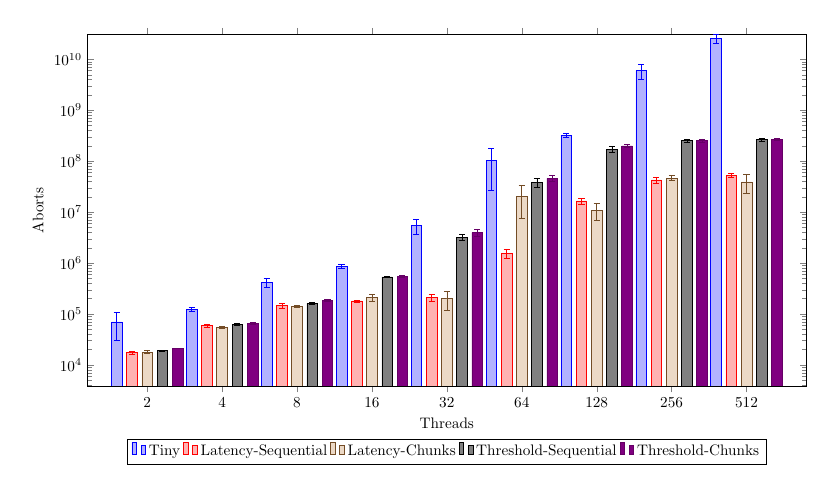
\begin{tikzpicture}[scale=0.55, baseline]
        \begin{axis}[
            ymode=log,
            width=1.5 \linewidth,
            height=0.8 \linewidth,
            %media de tempo intruder
            ybar=3pt,
            %enlargelimits=0.10,
            legend style={at={(0.5,-0.15)}, anchor=north, legend columns=-1},
            ylabel=Aborts,
            xlabel=Threads,
            symbolic x coords={1, 2, 4, 8, 16, 32, 64, 128, 256, 512},
            xtick=data,
            ymin=0,
            ymax=31000000000,
            bar width=7pt,
            % nodes near coords,
            nodes near coords align={vertical},
        ]
        \addplot+[error bars,y dir=both, y explicit] coordinates {
            (1,0.0)+-(1,0.0) (2,69940.4)+-(2,38859.442881235445) (4,123224.4)+-(4,10230.047558051723) (8,421702.0)+-(8,83144.47432752221) (16,858817.0)+-(16,70319.27963794851) (32,5482927.6)+-(32,1822574.306164838) (64,102125071.2)+-(64,75531726.60526115) (128,324906951.0)+-(128,25833176.356745664) (256,5976414236.0)+-(256,1965369780.1742249) (512,25331573456.2)+-(512,5125278647.27645) 
        };
        \addplot+[error bars,y dir=both, y explicit] coordinates {
            (1,0.0)+-(1,0.0) (2,17295.8)+-(2,884.117051074121) (4,58832.4)+-(4,5182.0950049183775) (8,145328.0)+-(8,14502.15570182585) (16,179942.6)+-(16,9939.803108713975) (32,213282.4)+-(32,33756.78063204487) (64,1563534.8)+-(64,303501.08637854987) (128,16550448.4)+-(128,2123035.5644618487) (256,42956098.2)+-(256,6012180.935710481) (512,52269879.0)+-(512,4755551.76397057)
        };
        \addplot+[error bars,y dir=both, y explicit] coordinates {
             (1,0.0)+-(1,0.0) (2,17786.7)+-(2,1249.259304548099) (4,54750.2)+-(4,2738.370420523856) (8,141273.5)+-(8,6123.819286197136) (16,209526.5)+-(16,34736.26421551402) (32,201599.3)+-(32,81127.76465680539) (64,20569626.4)+-(64,12875680.754533986) (128,10897558.0)+-(128,4040389.7657925775) (256,46668204.777777776)+-(256,5450523.901092766) (512,39389491.0)+-(512,16022591.920577014) 
        };
        \addplot+[error bars,y dir=both, y explicit] coordinates {
            (1,0.0)+-(1,0.0) (2,19074.2)+-(2,369.0059078117856) (4,61648.4)+-(4,2902.3763091646124) (8,161693.8)+-(8,9525.331540686655) (16,536547.4)+-(16,18869.180433712536) (32,3237316.8)+-(32,385306.9331768636) (64,38103581.6)+-(64,7477543.014654762) (128,171013189.4)+-(128,21848968.54501459) (256,256035773.6)+-(256,17482704.25370147) (512,263634097.2)+-(512,12981014.911830684)
        };
        \addplot+[error bars,y dir=both, y explicit] coordinates {
            (1,0.0)+-(1,0.0) (2,21093.1)+-(2,312.0) (4,64726.72)+-(4,3041.77) (8,183647.1)+-(8,8673.62) (16,544787.54)+-(16,23782.8) (32,3980021.4)+-(32,552484.0028907986) (64,45836278.2)+-(64,6287845.41) (128,199521897.4)+-(128,10431600.060439752) (256,254781534.6)+-(256,19017136.502195936) (512,266950650.75)+-(512,14874593.300939599)
        };
        \legend {Tiny, Latency-Sequential, Latency-Chunks, Threshold-Sequential, Threshold-Chunks}
        \end{axis}
        \end{tikzpicture}
    \caption{Aborts do benchmark Vacation variando o número de \emph{threads}.}
    \label{vacation_abort}

\end{figure}

Por fim, o experimento Yada~\ref{yada_abort} também apresentou para todos os testes uma redução expressiva no número de aborts. Onde pode ser observado uma redução de 99\% no teste Latency-Sequential com 512 threads. A menor redução de aborts apresentada no escalonador junto ao benchmark Yada foi de 97\% e ocorreu com a configuração Latency-Chunks com 2 threads.

\begin{figure}[!ht]
    \centering
        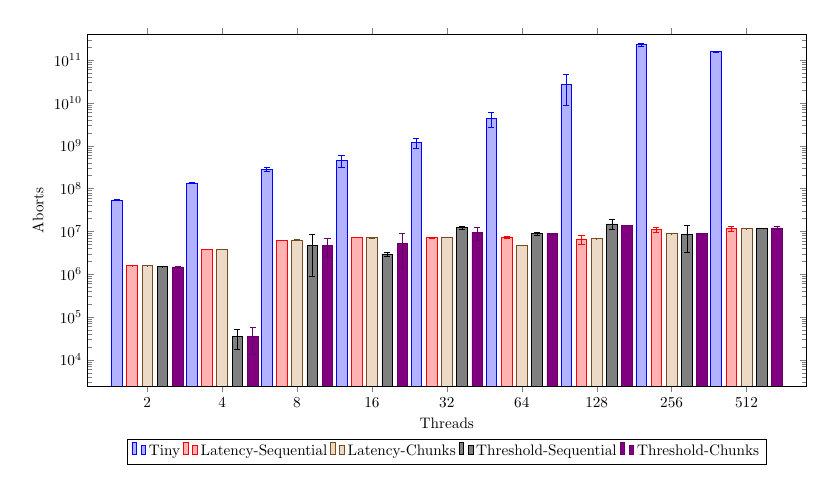
\begin{tikzpicture}[scale=0.55, baseline]
        \begin{axis}[
            ymode=log,
            width=1.5 \linewidth,
            height=0.8 \linewidth,
            %media de tempo intruder
            ybar=3pt,
            %enlargelimits=0.10,
            legend style={at={(0.5,-0.15)}, anchor=north, legend columns=-1},
            ylabel=Aborts,
            xlabel=Threads,
            symbolic x coords={1, 2, 4, 8, 16, 32, 64, 128, 256, 512},
            xtick=data,
            ymin=0,
            ymax=400000000000,
            bar width=7pt,
            % nodes near coords,
            nodes near coords align={vertical},
        ]
        \addplot+[error bars,y dir=both, y explicit] coordinates {
            (1,0.0)+-(1,0.0) (2,53805739.2)+-(2,945974.4856792702) (4,136025541.2)+-(4,4837342.13) (8,281305083.6)+-(8,28618515.67361887) (16,455944205.2)+-(16,138166587.07) (32,1205121875.2)+-(32,315403375.80832976) (64,4297295036.4)+-(64,1609418223.03) (128,27371816768.6)+-(128,18399453268.002537) (256,230017372308.6)+-(256,19982225506.96) (512,156775482845.2)+-(512,5418181512.20) 
        };
        \addplot+[error bars,y dir=both, y explicit] coordinates {
            (1,0.0)+-(1,0.0) (2,1580633.2)+-(2,8478.500749542929) (4,3800972.6)+-(4,20650.110223434644) (8,6149664.4)+-(8,75882.93103880476) (16,7207458.2)+-(16,106075.91092684522) (32,7097792.4)+-(32,149914.3555148739) (64,7245601.6)+-(64,297306.3815181907) (128,6626592.6)+-(128,1601916.1098185633) (256,11035923.666666666)+-(256,1354186.7993902795) (512,11463741.25)+-(512,1422857.6912357355)
        };
        \addplot+[error bars,y dir=both, y explicit] coordinates {
             (1,0.0)+-(1,0.0) (2,1586885.6)+-(2,17013.20809959133) (4,3864768.25)+-(4,23733.99245149244) (8,6283745.6)+-(8,79485.5) (16,7192878.4)+-(16,178424.65) (32,7378729.9)+-(32,18573.11) (64,4723078.0)+-(64,3928.0) (128,6736182.0)+-(128,37123.3) (256,8828877.0)+-(256,12847.0) (512,11637482.0)+-(512,82034.0) 
        };
        \addplot+[error bars,y dir=both, y explicit] coordinates {
            (1,0.0)+-(1,0.0) (2,1502389.8)+-(2,8336.5398735266599) (4,34570.6)+-(4,17081.853735470282) (8,4673390.0)+-(8,3789634.775837482) (16,2964970.8)+-(16,290439.4272928145) (32,12301780.8)+-(32,1054972.452489657) (64,9002166.4)+-(64,735560.767845634) (128,14938022.8)+-(128,3727246.128412794) (256,8642330.0)+-(256,5465830.0) (512,11928378.731)+-(512,74928.0)
        };
        \addplot+[error bars,y dir=both, y explicit] coordinates {
            (1,0.0)+-(1,0.0) (2,1483981.3)+-(2,5287.71) (4,34983.38)+-(4,21305.7) (8,4728374.12)+-(8,2263748.1) (16,5260517.0)+-(16,3862894.25) (32,9462941.0)+-(32,3192100.38) (64,8837692.27)+-(64,384722.0) (128,13729279.5)+-(128,110344.5) (256,8874348.23)+-(256,63743.0) (512,11973628.0)+-(512,837874.02)
        };
        \legend {Tiny, Latency-Sequential, Latency-Chunks, Threshold-Sequential, Threshold-Chunks}
        \end{axis}
        \end{tikzpicture}
    \caption{Aborts do benchmark Yada variando o número de \emph{threads}.}
    \label{yada_abort}

\end{figure}

Os resultados apresentam para maioria dos experimentos uma redução significativa do número de abort quando utilizado o escalonador proposto. Ao ultrapassar o número de threads hyper threading disponíveis na arquitetura utilizada todos os benchmarks apresentaram uma redução significativa no número de aborts, com melhor caso chegando até 99\% de redução dos aborts.

\section{Discussão}

Para maioria dos benchmarks o tempo de execução e número de aborts obtiveram melhor desempenho utilizando o LTMS, estes resultados possuem em seu melhor cenário uma redução de 96\% do tempo de execução e 99\% do número de aborts. Porém, alguns benchmarks obtiveram resultados piores com o LTMS em diferentes configurações quando comparados a TinySTM. Isto mostra a importância de entendermos a aplicação. Ter um escalonador capaz de entender melhor as características da aplicação e conhecer a arquitetura pode, como vimos na maioria dos benchmarks, obter resultados expressivos.

O LSTM apresentou seus melhores resultados com o benchmark Intruder. O Intruder possui uma alta contenção e suas transações possuem um tempo médio de execução. Os resultados do Intruder apresentaram redução no tempo de execução e no número de aborts para todos os cenários de threads. Estas características ajudam a prover um melhor mapeamento da aplicação onde o escalonador utiliza melhor o recurso de migração das threads.

O benchmark Kmeans apresentou um melhor tempo de execução até 128 threads, e teve um aumento no tempo de execução com 256 e 512 threads. Porém, este benchmark obteve uma redução no número de aborts para todos os cenários de threads. O Kmeans possui como característica uma baixa contenção e possui um tempo curto na duração da transação, outra característica da aplicação é que ela possui uma quantidade pequena de endereços, ou seja, todos os acessos são feitos em poucos endereços. Esta característica fez com que o LSTM realizasse mais migrações reduzindo o número de aborts e aumentando o tempo de execução. Para aplicações com estas características é importante manter o número de threads limitado às características da aplicação.

Os experimentos Labyrinth, Vacation e Yada apresentaram resultados melhores com o LTMS para a maioria dos cenários de threads. Estes benchmarks possuem em comum um alto tempo de execução dentro das transações.
%Porém apresentam algumas características distintas que influenciam os resultados. Vacation e Yada possuem contenção média e resultados parecidos,

As heurísticas desenvolvidas obtiveram resultados parecidos nos testes executados. Sendo que a heurística de migração Threshold apresenta um desempenho pior que a heurística Latency para aplicações com contenção média e quantidade média de endereços distintos acessados, como foi apresentado no experimento Yada.

É possível identificar que em alguns cenários de threads o LTMS obteve uma redução no número de aborts e não apresentou redução no tempo de execução. O LTMS obtém a serialização das threads conflitantes por meio da migração, para as aplicações que geram muita migração foram identificadas duas características. A primeira está na serialização total da aplicação, o que gera um tempo de execução semelhante a execução com 1 thread. A segunda característica identificada foi o aumento de overhead originado por migrações repetitivas. As heurísticas de migração buscam entender as aplicações e reduzir estas duas características limitando o número de migração. Porém para aplicações com baixa contenção e que utilizam uma quantidade pequena de endereços, utilizar uma heurística mista que avalie o índice de contenção e o número de threads ativos pode reduzir o tempo de execução evitando o excesso de migração.

\chapter{Conclusão}
\label{chapter::conclusao}

Muitos estudos de STM apresentam escalonadores transacionais que focam em reduzir o número de conflitos por meio da serialização das transações, reduzindo as threads ativas na aplicação ou bloqueando as transações conflitantes. Reduzir o número de conflitos se mostra eficiente para melhorar o desempenho, mas em arquiteturas multicores atuais com hierarquias de memória complexas também é importante considerar onde a posição de memória utilizada está localizada e por qual núcleo ela é acessada.

O entendimento da arquitetura utilizada é importante para o desempenho, melhorando a localidade e reduzindo a latência dos acessos à memória. As aplicações que utilizam STM oferecem oportunidades interessantes para entendimento da arquitetura e aplicação, pois em tempo de execução o STM fornece informações precisas sobre as áreas de memória que são compartilhadas entre threads, seus respectivos endereços e a intensidade com que cada endereço é acessado pelas threads. A partir do mapeamento destas informações este trabalho desenvolveu um escalonador NUMA-Aware que permite a migração de threads entre as filas de execução.

A principal contribuição desta dissertação está no projeto de um escalonador de STM modular que considera a arquitetura utilizada. O escalonador intitulado~\emph{LTMS} foi apresentado no capítulo~\ref{chapter::ltms}. O LTMS compreende a arquitetura utilizada e sua aplicação, para isto, o escalonador utiliza coleta de dados das threads e de suas transações em tempo de execução. O LTMS fornece um mecanismo de distribuição inicial de threads, criação de filas, e migração de threads conflitantes entre as filas existentes. Este mecanismo busca otimizar o desempenho de aplicações paralelas, reduzindo conflitos repetidos por meio da migração de threads agrupando as threads conflitantes na mesma fila.
% A etapa de inicialização do escalonador contribui com um sistema de filas individuais para os \emph{cores}, apresentado na sessão~\ref{inicializacao}, na qual para executar a distribuição das threads entre estas filas podemos utilizar diferentes heurísticas. Este trabalho apresentou duas heurísticas de distribuições. Estas heurísticas buscam distribuir inicialmente estas threads entre as filas disponíveis para entender o comportamento do número inicial de conflitos existentes na aplicação e comportamento do acesso à memória.

% Em tempo de execução o escalonador contribui com um mecanismo para coleta de dados da STM, apresentado na sessão~\ref{coleta}, onde são montadas duas matrizes uma de comunicação e uma de endereços. A matriz de comunicação fornece insumos sobre a quantidade de acessos aos endereços em comum entre threads. A matriz de endereços apresenta o endereço em comum mais acessado entre duas threads. Além destas matrizes, são coletadas informações sobre a latência de acesso à memória entre os nós disponíveis na arquitetura e a quantidade de aborts e commits que ocorreram em cada thread. Estas informações são insumos para compreender a arquitetura e a aplicação e são fundamentais para tomada de decisão na etapa de migração de threads do escalonador.

% A última contribuição deste trabalho está em um sistema de migração de threads, apresentado na sessão~\ref{migracao}, que é ativado apenas após a ocorrência de um abort da aplicação. O escalonador identifica a thread que gerou o abort, e com base nas informações previamente coletadas identifica para qual fila deve migrar está thread. O escalonador tem como base migrar a thread para uma fila na qual exista uma thread com maior número de acessos em comum à memória. Para tomada de decisão, se uma thread deve ou não ser migrada, é possível utilizar diferentes heurísticas para estudo, nesta dissertação foram utilizadas duas heurísticas. A primeira baseia-se na relação entre abort e commit, quando esta relação fica acima de um valor pré definido temos um indicativo de uma aplicação com alto índice de conflitos e o escalonador efetua a migração com intuito de reduzir os conflitos na aplicação. Para identificar o valor limiar utilizado neste trabalho foram executados testes onde chegamos ao limiar de 0.8, que indica que com 80\% na relação de aborts e commits a thread deve ser migrada. A segunda heurística utiliza o custo da latência no acesso à memória como parâmetro para efetuar a migração, onde se a fila atual que o thread executa possuir latência maior que a fila para qual desejamos migrar o escalonador efetua a migração, está heurística busca reduzir o custo de latencia gasto na aplicação.

Esta dissertação também apresenta como contribuição a prototipação do escalonador LTMS, utilizando a biblioteca de STM TinySTM. O LTMS por ser modular permite a criação e configuração de diferentes estratégias de distribuição e migração de threads, o que permite ampliar seu estudo e avaliar diferentes características. Esta prototipação inclui duas configurações para estratégia de distribuição de threads e duas heurísticas de migração, que buscam entender o comportamento do escalonador para diferentes aplicações.

Por fim, este trabalho apresenta como contribuição à análise de desempenho do LTMS comparado a TinySTM utilizando os benchmarks do conjunto de benchmarks STAMP. Os experimentos foram rodados com o escalonador com ambas configurações de heurísticas desenvolvidas, como apresentado no capítulo~\ref{chapter::experimentos}, e comparados com a biblioteca original de TinySTM. Concluímos que as aplicações utilizando LTMS apresentam para maioria dos cenários e configurações uma redução no tempo de execução e número de aborts. Sendo que o LTMS quando comparado com a TinySTM obteve uma redução de até 96\% do tempo de execução e 99\% do número de aborts com benchmark Intruder utilizando configuração Latency-Sequential.

\section{\textbf{Trabalhos futuros}}

A pesquisa apresentada neste trabalho pode ser estendida das seguintes formas:

\begin{itemize}
\item \emph{Comparação do LTMS com outros escalonadores}: Para trabalhos futuros pretendemos executar testes para avaliar o desempenho de tempo de execução e número de aborts com outros benchmarks apresentados na literatura;

 \item \emph{Novas estratégias de distribuição}: O LTMS permite explorar distintas estratégias de distribuição de threads ao inicializar a aplicação. Com isso é importante avançarmos nos estudos para explorar diferentes formas de distribuição e compará-las. As distintas características entre as estratégias de distribuição podem ser exploradas em trabalhos futuros;

 \item \emph{Heurística de migração híbrida}: O LTMS permite aplicar duas heurísticas de migração, uma com foco no índice de contenção e outra com foco na latência de acesso à memória, mas o escalonador permite que estas heurísticas possam ser utilizadas juntas para aperfeiçoar o sistema de migração, buscando a redução da contenção e otimização do acesso à memória para reduzir a latência da aplicação; e

 \item \emph{Impacto energético dos escalonadores de STM}: Os trabalhos atuais focam no impacto que os escalonadores possuem sobre o desempenho de tempo e redução de conflitos. Um aspecto a ser abordado em trabalhos futuros pode ser o impacto que escalonador com consciência da arquitetura, como o LTMS, possuem em relação ao custo energético em relação a outros escalonadores.
\end{itemize}

O escalonado LTMS, desenvolvido nesta dissertação, pode ser estendido permitindo que estas características sejam avaliadas em trabalhos futuros. Assim, podemos seguir com o desenvolvimento do LTMS contribuindo e explorando outros aspectos da área.

\bibliographystyle{abnt}
\bibliography{bibliografia} 

% Apêndices (Opcional) - Material produzido pelo autor
% \apendices
% \chapter{Um Apêndice}

% Anexos (Opcional) - Material produzido por outro
% \anexos
% \chapter{Um Anexo}

% \chapter{Outro Anexo}

% Faz a capa do CDROM
% \makecover

\end{document}

